\documentclass{article}
% Packages used
% Packages
\usepackage{amssymb,amsmath,amsthm,bbm}
\usepackage{verbatim,float,url,dsfont}
\usepackage{graphicx,subfigure,psfrag}
\usepackage{algorithm,algorithmic}
\usepackage{mathtools,enumitem}
\usepackage{multirow}
\usepackage{ragged2e}
\usepackage{xr-hyper}
\usepackage{array}

\usepackage[colorlinks=true,citecolor=blue,urlcolor=blue,linkcolor=blue]{hyperref}
\usepackage[margin=1in]{geometry}
\usepackage[round]{natbib}

\usepackage[utf8]{inputenc} % allow utf-8 input
\usepackage[T1]{fontenc}    % use 8-bit T1 fonts
\usepackage{booktabs}       % professional-quality tables
\usepackage{nicefrac}         % compact symbols for 1/2, etc.
\usepackage{microtype}      % microtypography
\usepackage{pdflscape}

\ifdefined\TimesFont 
\usepackage{times} % use times font
\fi

\ifdefined\ParSkip 
\usepackage{parskip} % use par skip
\fi

% Place page number
\def\fillandplacepagenumber{%
 \par\pagestyle{empty}%
 \vbox to 0pt{\vss}\vfill
 \vbox to 0pt{\baselineskip0pt
   \hbox to\linewidth{\hss}%
   \baselineskip\footskip
   \hbox to\linewidth{%
     \hfil\thepage\hfil}\vss}}
     
% Theorems and such
\newtheorem{theorem}{Theorem}
\newtheorem{lemma}{Lemma}
\newtheorem{corollary}{Corollary}
\newtheorem{proposition}{Proposition}
\theoremstyle{definition}
\newtheorem{remark}{Remark}
\newtheorem{definition}{Definition}

% Assumption
\newtheorem*{assumption*}{\assumptionnumber}
\providecommand{\assumptionnumber}{}
\makeatletter
\newenvironment{assumption}[2]{
  \renewcommand{\assumptionnumber}{Assumption #1#2}
  \begin{assumption*}
  \protected@edef\@currentlabel{#1#2}}
{\end{assumption*}}
\makeatother

% Widebar
\makeatletter
\newcommand*\rel@kern[1]{\kern#1\dimexpr\macc@kerna}
\newcommand*\widebar[1]{%
  \begingroup
  \def\mathaccent##1##2{%
    \rel@kern{0.8}%
    \overline{\rel@kern{-0.8}\macc@nucleus\rel@kern{0.2}}%
    \rel@kern{-0.2}%
  }%
  \macc@depth\@ne
  \let\math@bgroup\@empty \let\math@egroup\macc@set@skewchar
  \mathsurround\z@ \frozen@everymath{\mathgroup\macc@group\relax}%
  \macc@set@skewchar\relax
  \let\mathaccentV\macc@nested@a
  \macc@nested@a\relax111{#1}%
  \endgroup
}
\makeatother

% Min and max 
\DeclareMathOperator*{\argmin}{argmin}
\DeclareMathOperator*{\argmax}{argmax}
\DeclareMathOperator*{\minimize}{minimize}
\DeclareMathOperator*{\maximize}{maximize}
\DeclareMathOperator*{\find}{find}
\DeclareMathOperator{\st}{subject\,\,to}

% Other operators
\DeclareMathOperator{\Cov}{Cov}
\DeclareMathOperator{\Var}{Var}
\DeclareMathOperator{\dm}{dim}
\DeclareMathOperator{\col}{col}
\DeclareMathOperator{\row}{row}
\DeclareMathOperator{\nul}{null}
\DeclareMathOperator{\rank}{rank}
\DeclareMathOperator{\nuli}{nullity}
\DeclareMathOperator{\spa}{span}
\DeclareMathOperator{\sign}{sign}
\DeclareMathOperator{\supp}{supp}
\DeclareMathOperator{\diag}{diag}
\DeclareMathOperator{\aff}{aff}
\DeclareMathOperator{\conv}{conv}
\DeclareMathOperator{\dom}{dom}
\DeclareMathOperator{\tr}{tr}
\DeclareMathOperator{\df}{df}

% Other shortcuts 
\def\R{\mathbb{R}}
\def\C{\mathbb{C}}
\def\E{\mathbb{E}}
\def\P{\mathbb{P}}
\def\T{\mathsf{T}}
\def\half{\frac{1}{2}}
\def\df{\mathrm{df}}
\def\hy{\hat{y}}
\def\hf{\hat{f}}
\def\hmu{\hat{\mu}}
\def\halpha{\hat{\alpha}}
\def\hbeta{\hat{\beta}}
\def\htheta{\hat{\theta}}
\def\indep{\perp\!\!\!\perp}
\def\th{^{\textnormal{th}}}

\def\cA{\mathcal{A}}
\def\cB{\mathcal{B}}
\def\cD{\mathcal{D}}
\def\cE{\mathcal{E}}
\def\cF{\mathcal{F}}
\def\cG{\mathcal{G}}
\def\cK{\mathcal{K}}
\def\cH{\mathcal{H}}
\def\cI{\mathcal{I}}
\def\cL{\mathcal{L}}
\def\cM{\mathcal{M}}
\def\cN{\mathcal{N}}
\def\cP{\mathcal{P}}
\def\cS{\mathcal{S}}
\def\cT{\mathcal{T}}
\def\cW{\mathcal{W}}
\def\cX{\mathcal{X}}
\def\cY{\mathcal{Y}}
\def\cZ{\mathcal{Z}}

 \def\given{\, \vert\, }

\def\TimesFont{} 
\graphicspath{{gfx/}}

\newcommand{\beginsupplement}{
  \setcounter{table}{0}  
  \renewcommand{\thetable}{S\arabic{table}} 
  \setcounter{figure}{0} 
  \renewcommand{\thefigure}{S\arabic{figure}}
  \setcounter{section}{0} 
  \renewcommand{\thesection}{S\arabic{section}}
}
\font\supptitlefont=cmr12 at 16pt 
\newcommand{\attn }[1]{\textcolor{red}{ATTN: #1}}
     
\begin{document}
\title{Retrospective estimation of latent COVID-19 infections over the pandemic in US states}
\author{Rachel Lobay, Maria Jahja, Ajitesh Srivastava, Ryan J.\ Tibshirani, Daniel J.\ McDonald}
\date{Version: \today}
\maketitle

\begin{abstract}
The true timing and magnitude of COVID-19 infections are of interest to both the public
and to public health, but these are challenging to pin down for a variety of data-driven
and methodological reasons. Nevertheless, accurate estimates of latent COVID-19 
infections can improve our understanding 
of the true size and scope of the pandemic and provide an indication of disease 
patterns and burden over time. Therefore, we estimate daily incident infections 
for each \US\ state. Our methods first deconvolve reported COVID-19 cases to 
their infection onset. We then use a serology-driven model to scale these 
deconvolved cases to unreported infections. Unlike existing approaches,
our approach is state-specific, incorporates several variant-specific incubation
periods, and accounts for reinfections. From its application to the gold standard case
data, we find a disease burden that appears earlier and more extensively than indicated
by cases alone. In addition, we observe similar epidemic patterns in surges and
periods of waning observed in clusters of neighbouring states. Our findings help to 
better understand the impact of the pandemic in the \US\ at the level of the state. 

\end{abstract}

\section{Introduction}

Reported COVID-19 cases are a staple in tracking the pandemic at varying
geographic resolutions such as national, state and county levels
\citep{dong2020interactive, nyt2020corona, wp2020tracking}. Yet, for every case
that is eventually reported to public health, several infections are likely to
be missed. To see why, it is important to understand who's cases are being reported and
 what differentiates them from the unreported cases. Refer to
\autoref{fig:chain_events_onset_report} for an illustration of the path of a
symptomatic infection that is eventually reported to public health. 

Using this figure, we can discern a number of sources of bias in the reporting
pipeline. For instance, diagnostic testing mainly targets symptomatic
individuals; thus, infected individuals exhibiting little to no symptoms are
likely to be missed \citep{cdc2022estimated}. In addition, testing practices,
availability, and uptake vary across space and time \citep{pitzer2021impact,
ecdc2020strategies, hitchings2021usefulness}. Finally, cases provide a belated
view of the pandemic's progression because they are subject to delays due to the
viral incubation period, the speed and severity of symptom onset, laboratory
confirmation, test turnaround times, and submission to public health
\citep{pellis2021challenges, wash2020dash}. For these reasons, reported cases
are a lagging indicator of the course of the pandemic. Furthermore, they do not
represent the actual number of new infections that occur on a given day as
indicated by exposure to the pathogen. Since there is no large-scale surveillance
effort in the United States that reliably tracked symptom onset, let alone infection onset,
ascertaining the onset of infections is challenging.

\begin{figure}[!tb]
\centering
    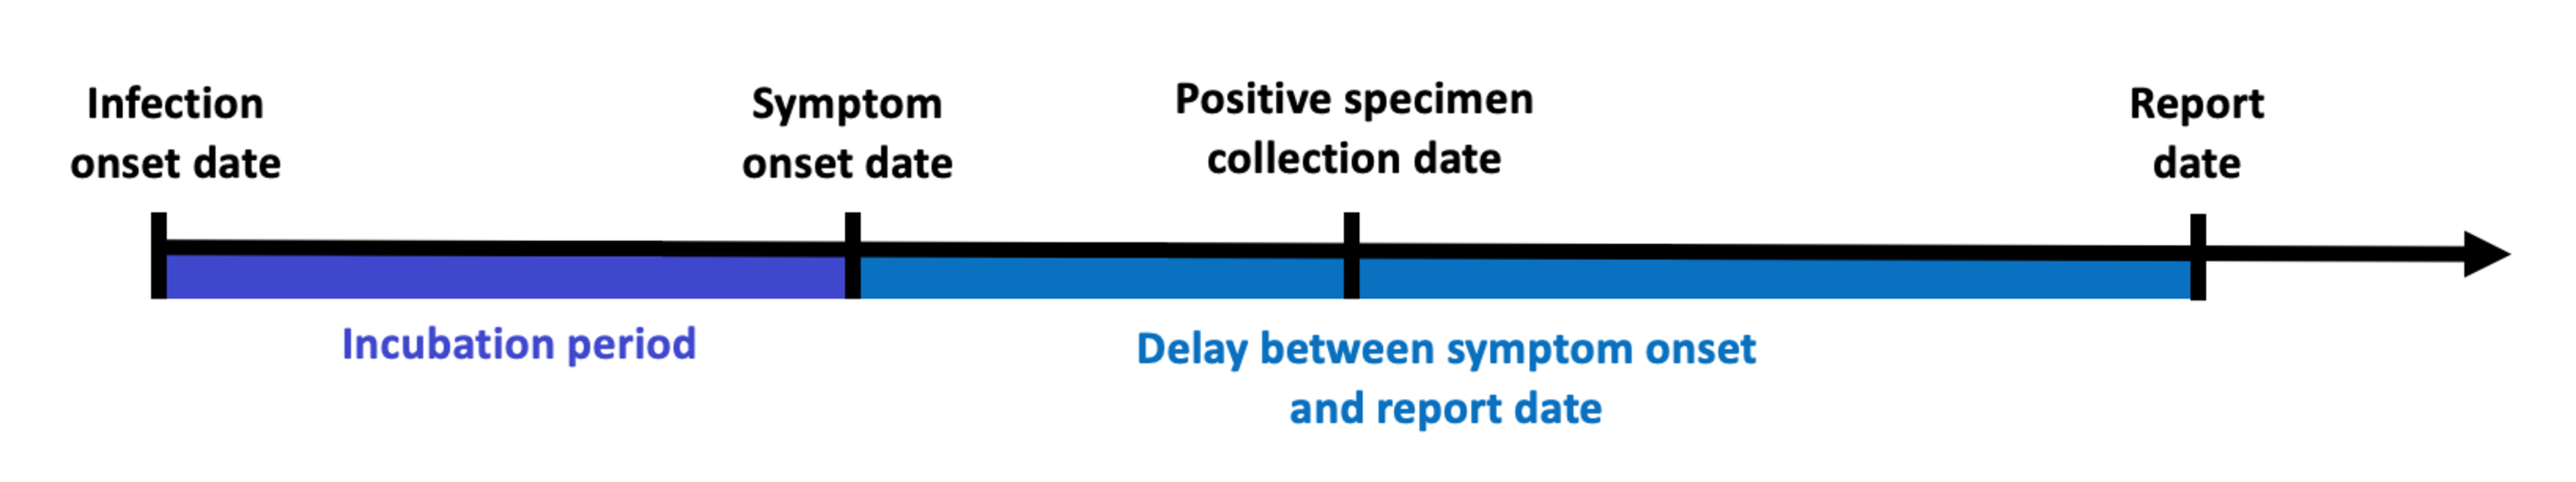
\includegraphics[width=.99\textwidth]{Chain_of_events_onset_report.pdf} 
    \caption{Idealized chain of events from infection onset to case report date 
    for a symptomatic infection that is eventually reported to public health.}
    \label{fig:chain_events_onset_report}
\end{figure}

% Importantly, all of these issues that are present in local health authority
% data are also present in the gold standard for case data from the JHU CSSE
% \citep{dong2020interactive, guidotti2022worldwide} because JHU scrapes case
% data from the local health authority dashboards \citep{jahja2022real}.
% Furthermore, the cases shown on the JHU CSSE Coronavirus Resource Center
% \citep{jhucsse2020covid} are those that have been disseminated to the public
% on a given day. 
% Our approach to estimate latent infections takes case data and estimates the 
% following...

Explaining the course of the pandemic and investigating the effects of
interventions, the burden facing various subgroups, and drawing insights for
future pandemics is challenging because the true spatial and temporal behaviour
is unknown. While reported cases provide some understanding of the disease
burden in a population, it is incomplete, delayed, and understates the true size
of the pandemic. Regardless of these difficulties, it is important to the public
and public health to perform a pandemic post-mortem and try to better estimate the
true extent of its effect---to attempt to capture the true size and impact of
the pandemic as much as we can. Estimates of daily incident infections are one
such way to measure this and can guide public and professional understanding of
the pandemic burden over space and time.

In this work, we provide a statistically justified reconstruction of
daily incident infections for each \US\ state from June 1, 2020 to November 29, 2021.
We achieve this by breaking the task of estimating infection onset
from report date into the more manageable parts of estimating the time from
infection to symptom onset, symptom onset to positive specimen collection,
and the time from positive specimen collection to report date (as
depicted in \autoref{fig:chain_events_onset_report}). Using state-level line list data, 
we construct time-varying delay distributions for the time from symptom onset to positive
specimen date and positive specimen to case report date. We then use 
variant-specific incubation period distributions in conjunction with these delay distributions to
deconvolve daily reported COVID-19 cases back to their infection onset.
The resulting infection estimates are adjusted to account for the unreported infections by
using seroprevalence data in a novel antibody prevalence model that is defined by its
ability to account for the waning of antibody detectability over time.  
We examine some features of our infection estimates and the implications of
using them rather than reported cases in assessing the impact of the pandemic.
We apply our infection estimates to get time-varying infection-hospitalization
ratios (IHRs) for each state and compare those to similarly derived
case-hospitalization ratios (CHRs).
% finding major spikes that correspond to the introduction of prominent new variants in both, but 
% higher ratios overall for cases.
While these analyses provide a glimpse into the utility of these
infection estimates, we believe that there is much more to be explored, and we hope that
our work will prove an important benchmark for others to undertake retrospective
analyses.

\section{Methods}

In what follows, we provide details on how we estimate the daily incident
infections for each state over the considered time period of June 1, 2020 to
November 29, 2021 and the data we used to achieve this. We start with a brief
introduction to each data source used and follow this with a description of each
major analysis task in the order they are performed.
\autoref{fig:cases_to_infect_flowchart} provides a visual summary of the data,
analysis tasks, and the relationships between them. The major analysis tasks this 
figure aims to convey are as follows: 
First, we estimate variant-specific incubation periods and two types of delay distributions
 for each day over the considered time period. Next, each incubation period and symptom
  onset to positive specimen delay distribution are joined using convolution to obtain
   variant-specific infection onset to positive specimen distributions for each time. Then
    two types of deconvolution are performed. We first deconvolve from case report to
     positive specimen date. We then deconvolve from positive specimen to report
      date by variant. The resulting infection estimates are aggregated across the variant
       categories, and adjusted to account for the unreported infections by using state-specific, 
       time-varying seroprevalence data in an antibody prevalence model. This lets us reach our 
       ultimate goal of obtaining daily incident infection estimates.
% Then, we can apply these estimates in a
% lagged correlation to hospitalizations to find the ``best'' lag between
% infection and hospitalization rates according to Spearman's rank-based correlation 
% and use this to compute time-varying IHRs for each state. 


\begin{figure}[!tb]
\centering
    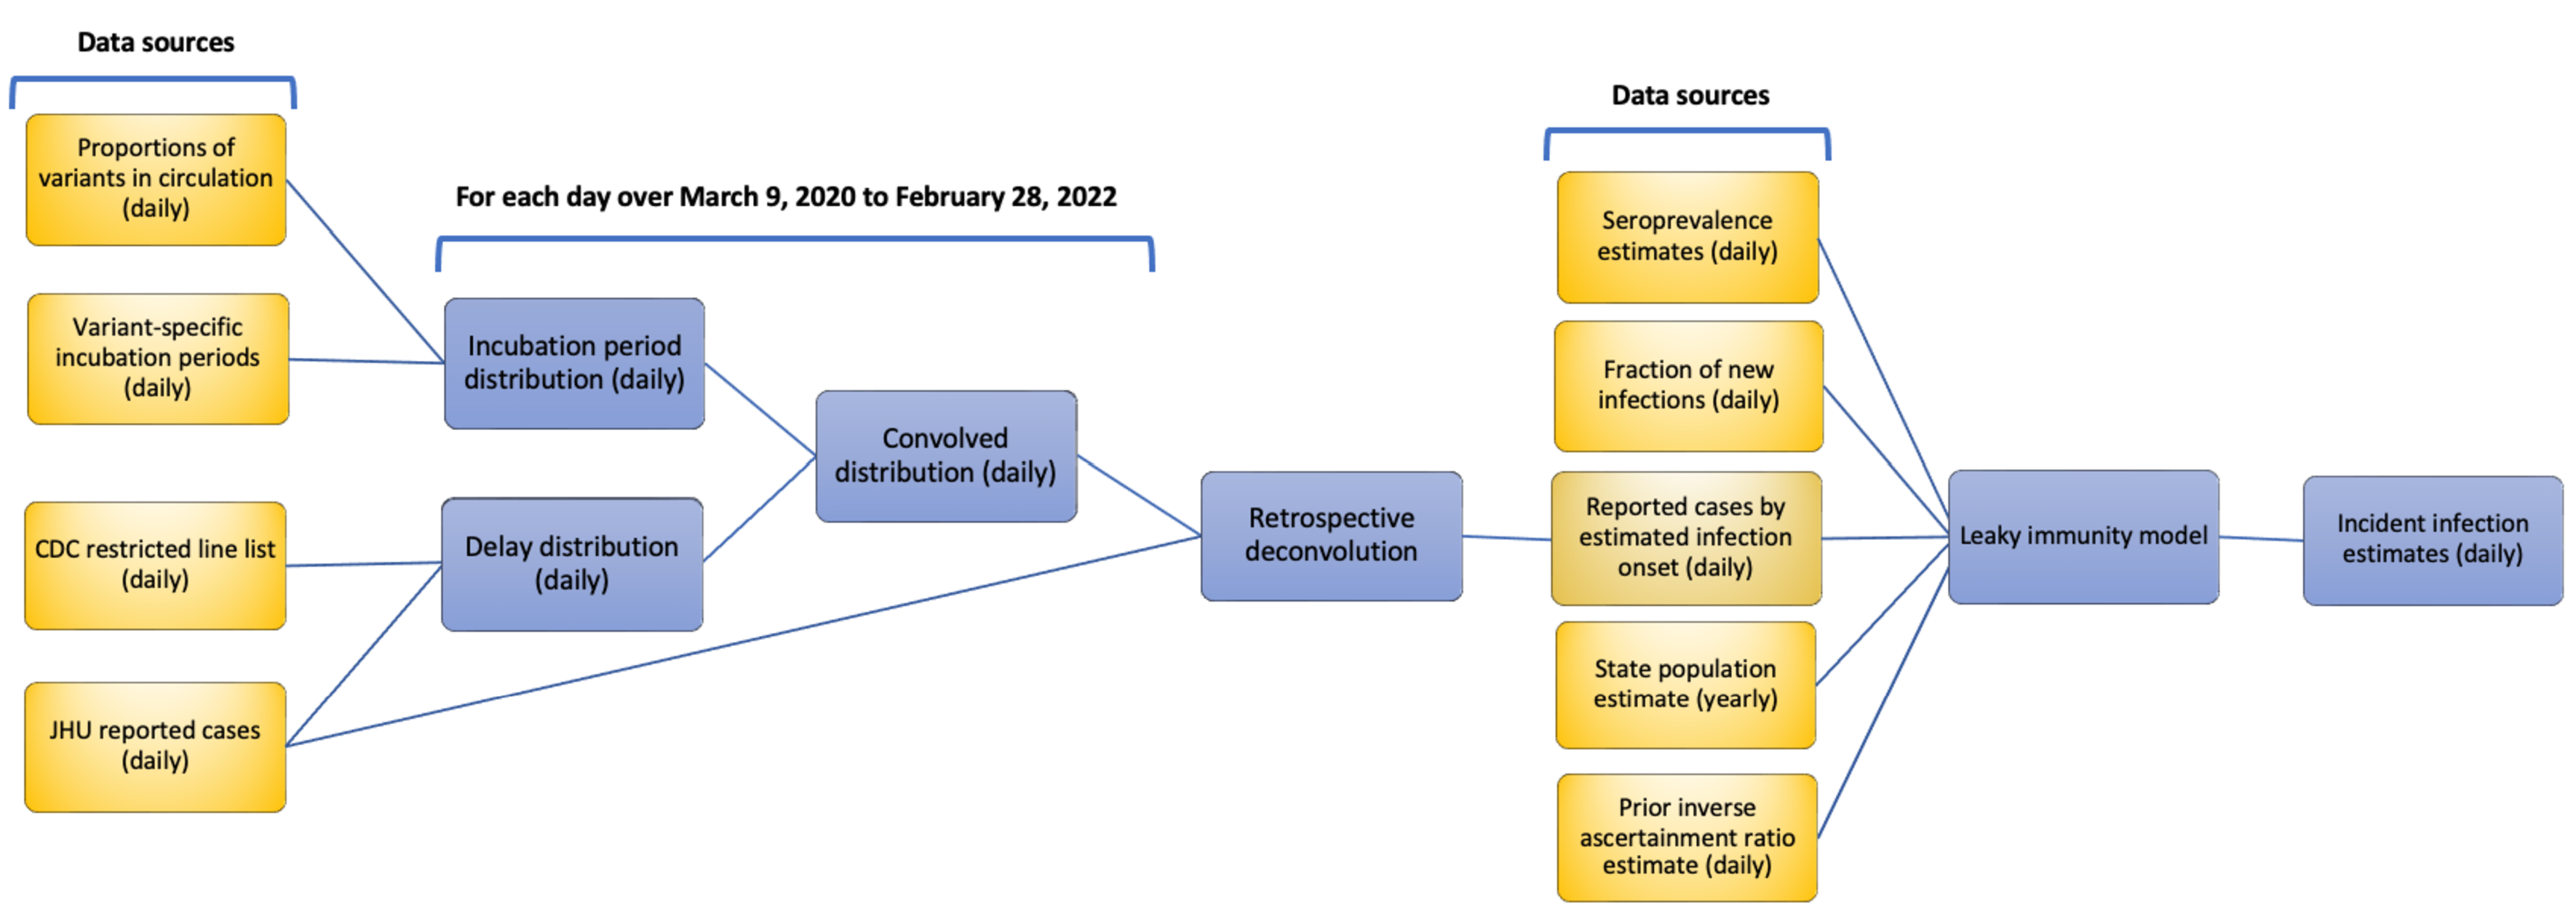
\includegraphics[width=.99\textwidth]{Reported_cases_to_infect_flowchart.pdf} 
    \caption{Flowchart of the inputted data and major analysis steps required 
    to get from reported cases to incident infection estimates for each day 
    over June 1, 2020 to November 29, 2021 for a state. Data sources are coloured 
    in yellow, while data analysis steps are coloured in blue. The data sources that
    do not stem from an analysis step are literature estimates.}
    \label{fig:cases_to_infect_flowchart}
\end{figure}


% Reasons why we should start from June 1, 2020 
% A list of reasons on why I settled on these start and end dates: 
% 1. Reinfections officially started occurring 2020-06-01 according to the data we?re using
% 2. sero measurements start in July 2020 for most states or later
% 3. the prior values for the inverse of the ascertainment ratio estimates are as of 2020-06-01
% 4.  the earliest hospitalizations for each state (that we use in the correlation analysis) 
% are also almost always in July, 2020. 
% So I am not convinced we should extrapolate multiple months away from the start or end for sero. 
% One month in either direction seems reasonable & doesn't overreach.

\subsection{Data} 

We obtain literature estimates of the variant-specific incubation periods
for the following eight variant categories: Ancestral, Alpha, Beta, Epsilon, Iota, 
Gamma, Delta, and Omicron.
For the Ancestral variants, we use the
literature estimates of the gamma distribution parameters \citep{tindale2020evidence}. 
For the Alpha, Beta, Gamma, Delta and Omicron variants, we use the
mean and standard deviation of the number of days of incubation as reported in
\citet{tanaka2022shorter, grant2022impact, ogata2022shorter}.\footnote{To clarify, 
we use the estimates for Alpha and Omicron from \citet{tanaka2022shorter}, those for
Beta and Gamma from \citet{grant2022impact}, and those for Omicron from
\citet{ogata2022shorter}.} Since the literature lacks reliable estimates for the incubation
period of the Epsilon and Iota variants, we use the
incubation period for Beta because Epsilon, Iota, and Beta are all
children from the same parent in the phylogenetic tree of the Nextstrain Clades
(as depicted in \citealp{hodcroft2021covariants}). 

To estimate the daily proportions of the variants circulating in each state, we
obtain the GISAID genomic sequencing data counts from CoVariants.org
\citep{hodcroft2021covariants, elbe2017data}.\footnote{The complete list of
EPI\_SET Identifiers that were used to produce the CoVariants data are provided
in the Acknowledgements section of their website
\citep{hodcroft2021covariants}.} Since these counts are biweekly totals, we apply
multinomial logistic regression using a third-order polynomial in time to get 
estimates of the daily proportions for the eight variant categories separately for each state.
% This relatively simple model was selected because it allows for exponential growth 
% and different rates by variant.
% Since these counts are biweekly totals, we use
% a simple convex optimization approach to interpolate daily numbers, where we
% enforce that the counts in each interval must sum to the right boundary (the
% biweekly total) and linear growth between the pairs of adjacent days. 

The COVIDcast API \citep{reinhart2021open} is used to retrieve the daily number
of new confirmed COVID-19 cases for each state that are based on reports from
the John Hopkins Center for Systems Science and Engineering (JHU CSSE,
\citealp{dong2020interactive}). From the same API, we also retrieve the daily
number of confirmed COVID-19 hospital admissions for each state that are
collected by the \US\ Department of Health and Human Services (HHS). Both
datasets are updated as of June 6, 2022.

We obtain de-identified patient-level line list data on COVID-19 cases from the
CDC. Although there are both public and restricted versions of the dataset
available containing the same patient records \citep{cdc2020casepub,
cdc2020caserestr}, the restricted dataset\footnote{The CDC does not take
responsibility for the scientific validity or accuracy of methodology, results,
statistical analyses, or conclusions presented.} is selected because it contains
information on the state of residence which is essential for constructing
state-specific delay distributions. Since the restricted dataset is updated
monthly and cases may undergo revision, we use a single version of it that was
released on June 6, 2022. We consider this version to be finalized in that it
well-beyond our study end date such that the dataset is unlikely to be subject
to further significant revisions.

In this dataset, the three key variables of interest are the dates of symptom
onset, positive specimen date and report to the CDC. 
Table~\ref{order_events_table} presents the percent of pairwise occurrences
 for the different possible permutations of events in the line list. 
Essentially, most cases follow the idealized ordering shown by
 \autoref{fig:chain_events_onset_report} and so we adhere to this construction 
 as much as possible. 

We observe that the line list is prone to
high percentages of missing data, notably with respect to our variables of
interest. Approximately 62.3\% of cases are missing the symptom onset 
date, 55.4\% are missing positive specimen date, and 8.96\% of cases 
are missing the report date. Relatedly, we faced the
fundamental issue that \citet{jahja2022real} described, in which cases with
missing report dates may be filled with their symptom onset date. On top of this, 
we have the additional factor
of positive specimen date to contend with. Previous correspondence with the 
CDC confirms that the imputation issue
extends to this variable as well. So it is possible that all three variables may be
 imputed with the same date for a case.
However, we only actually deal with select pairs of events; 
we do not use all three at once
in our construction of the delay distributions or anywhere else in our analysis.
Therefore, we restrict our investigation of missingness to the pairs of events. 
\autoref{fig:prop_cc_zero_delay} suggests that this issue impacts states differentially
due to the inconsistent proportions of zero delay between positive specimen and 
report date across states. 

Due to the contamination in the zero delay cases (the true extent of
which is unknown to us), we omit all such cases where the positive specimen and 
report dates have zero delay from our analysis.
We choose to allow for zero and negative delay for symptom onset to report because 
correspondence with the CDC confirms the distinct possibility that a person could 
test positive before symptom onset and it is a reasonable ordering to expect if, for 
example, the individual is aware that they have been exposed to an infected individual. 
We explain how we incorporated these variations in the ordering of events into our 
analysis in Section~\ref{delaystop}. 

\begin{figure}[!tb]
\centering
    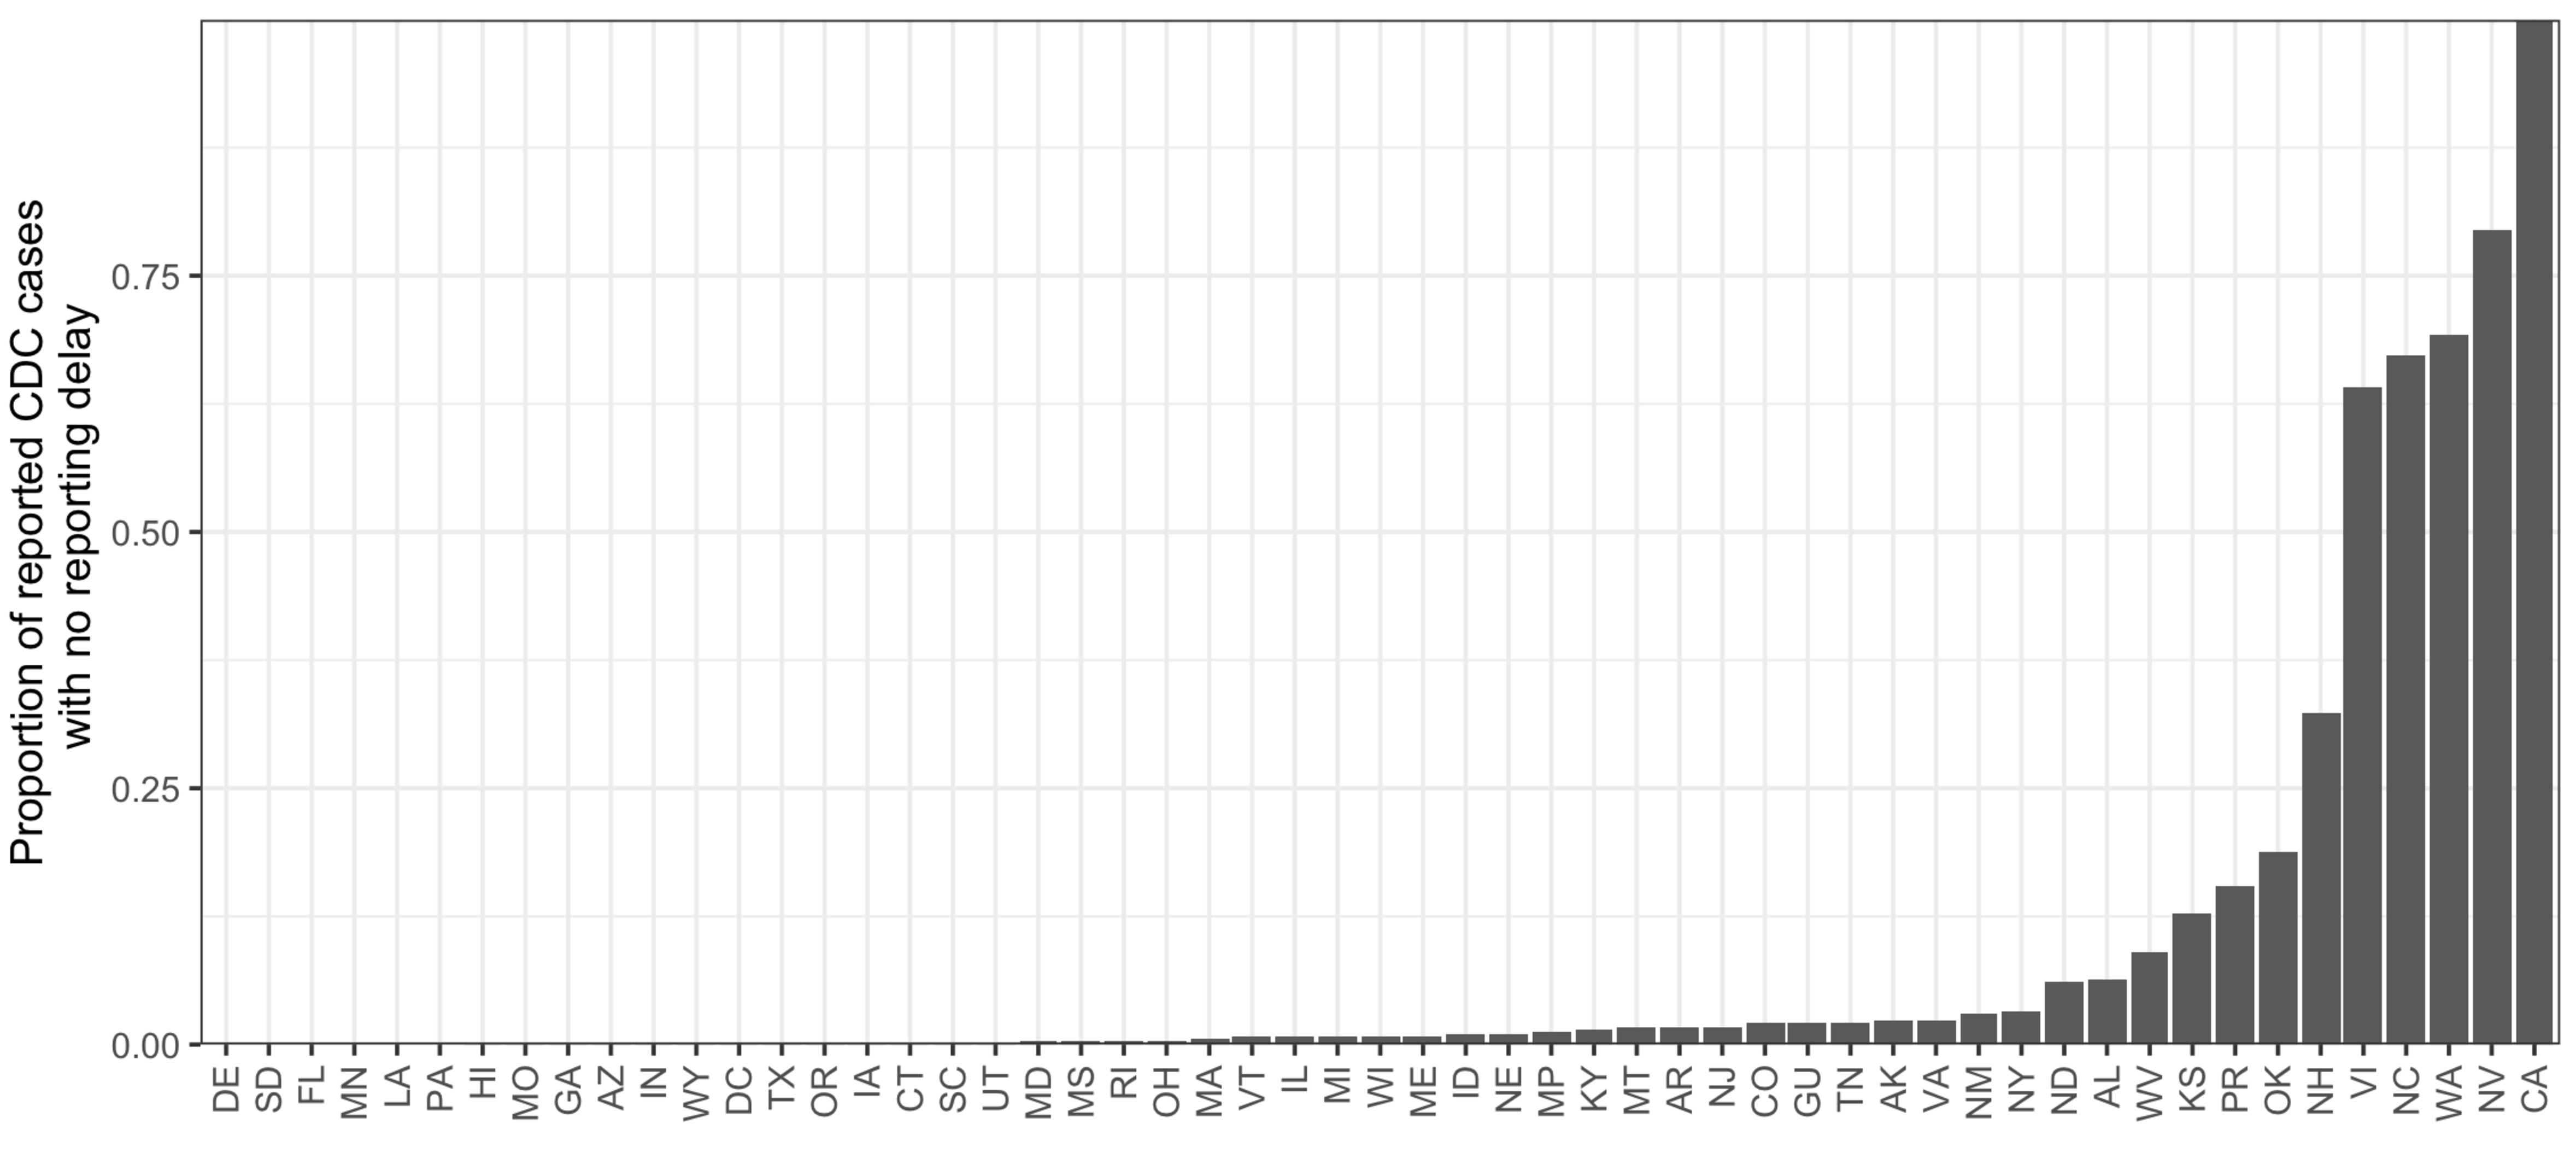
\includegraphics[width=.99\textwidth]{prop_cc_zero_delay.pdf}
    \caption{Proportions of complete cases with zero delay between positive specimen
     and report date in the restricted CDC line list dataset.}
    \label{fig:prop_cc_zero_delay}
\end{figure}

For the same release date, the restricted line list contains 74,849,225 cases
(rows) in total compared to 84,714,805 cases reported by the JHU CSSE; that is,
line list is missing about 10 million cases. The
extent that this issue impacts each state is shown in
\autoref{fig:prop_cc_cdc_vs_jhu}, from which it is clear the fraction of missing
cases is substantial for many states, often surpassing 50\%
\citep{jahja2022real}. In addition, the probability of being missing does not
appear to be the same for states, so there is likely bias introduced from using
the complete case line list data. We consider such bias to be unavoidable in our
analysis due to a lack of alternative line list sources.

\begin{figure}[!tb]
\centering
    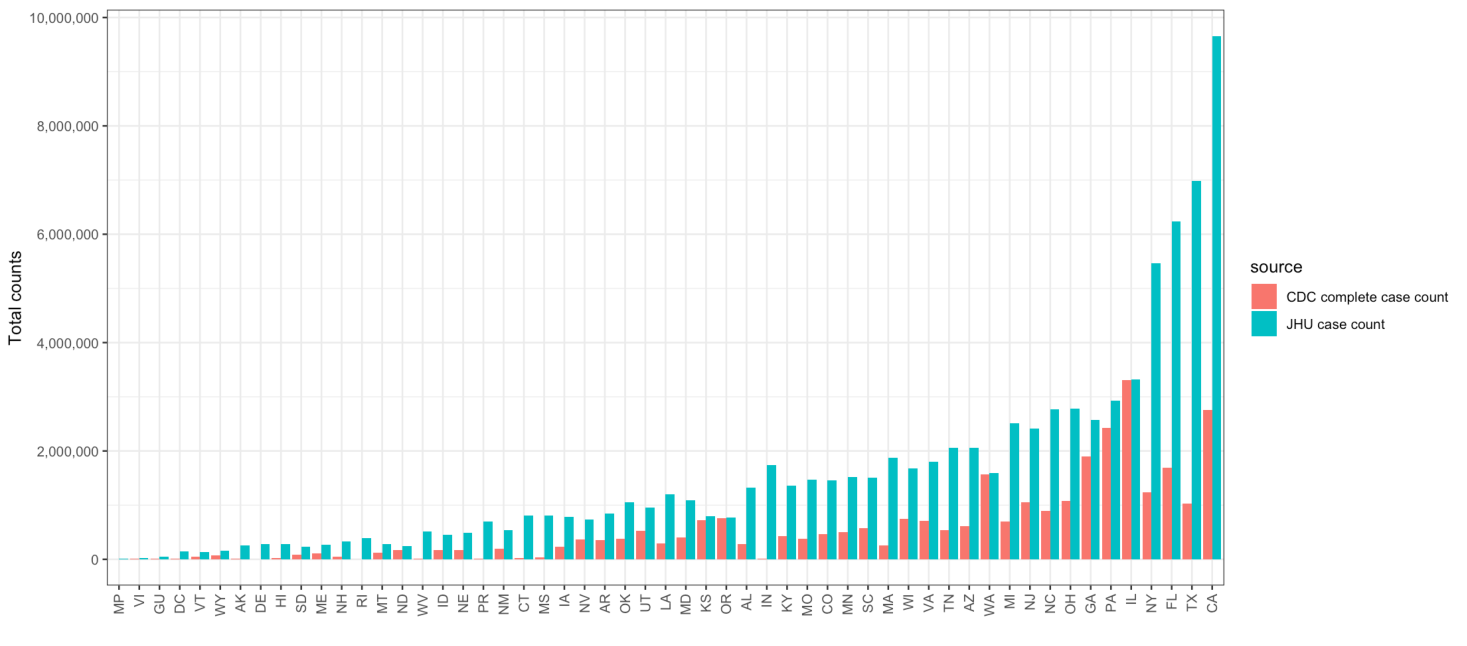
\includegraphics[width=0.99\textwidth]{prop_cc_cdc_vs_jhu.pdf} 
    \caption{Complete case counts by state in the CDC line list versus the 
    cumulative complete case counts from JHU CSSE as of June 6, 2022.
     All counts have been scaled by the 2022 state populations as of
     July 1, 2022 from \citet{uscensus2022annual}.}
    \label{fig:prop_cc_cdc_vs_jhu}
\end{figure}

In the line list, we observe unusual jarring spikes in reporting in 2020 compared
to 2021. Upon plotting by report date, we find that a few states are
contributing unusually large case counts on isolated days very late in the
reporting process (usually well beyond 50 days). We strongly suspect that
these large accumulations of cases over time are due breakdowns of the reporting
pipeline (which may be expected to occur more frequently in the year following
its instantiation than later in time). Such anomalies are not likely to be reliable
indicators of the delay from positive specimen to case report. Therefore, we devise
a simple, ad hoc approach to detect and prune these reporting backlogs.

First, we obtain the part of the line list intended for the positive specimen to case
 report delay estimation, where both such dates are present and where zero and
  negative delay cases have been omitted. 
Then, for each of the three dates of June 1, September 1, and
December 1, 2020, we bin the reporting delays occurring
from 50 days up to the maximum observed delay. For each bin, we obtain
the total delay count for each state. We check whether each count on the
log scale is at least the median (for the bin) plus 1.5 times the
interquartile range and retain only those that exceed this criterion as potential
candidates for pruning. Next, we compute the counts by report date for each
candidate state. If there is a report date with a count greater than or equal to
the pre-specified threshold, then we remove those cases from the line list.
Based on inspection and intuition, we set the threshold to 2000 for the
first two bins, and then lower it to 500 for the remaining bins. 
A similar trial and error approach is used to set the bin size (to 50 days). % Area for sensitivity
% analysis? Also, could discuss the choice of using only 3 dates 

To estimate the proportion of the population in each state with evidence of
previous infection across time, we use two major seroprevalence surveys that
were led by the CDC: the 2020--2021 Blood Donor Seroprevalence Survey and the
Nationwide Commercial Lab Seroprevalence Survey \citep{cdc2021blood,
cdc2021comm}. In the former, the CDC collaborated with 17 blood collection
organizations in the largest nationwide COVID-19 seroprevalence survey to date
\citep{cdc2021blood}. The blood donation samples were used to construct monthly
seroprevalence estimates for nearly all states from July 2020 to December 2021
\citep{jones2021estimated}. In the latter survey, the CDC collaborated with two
private commercial laboratories and used blood samples to test for the
antibodies to the virus from people that were in for routine or clinical
management (presumably unrelated to COVID-19, \citealp{bajema2021estimated}). The
resulting dataset contains seroprevalence estimates for a number of multi-week
collection periods starting in July 2020 to February 2022. 

Both datasets are based on repeated, cross-sectional studies that aimed, at
least in part, to estimate the percentage of people who were previously infected
with COVID-19 using the percentage of people from a convenience sample who had
antibodies against the virus \citep{bajema2021estimated, cdc2020data,
jones2021estimated}. Adjustments were made in both for age and sex to account
for the demographic differences between the sampled and the target populations.
However, both datasets are incomplete and they differ in the number and the
timing of the data points for each state (\autoref{fig:sero_blood_comm_compar}).
Such limitations indicate that reliance upon only one seroprevalence
survey is inadvisable.
For example, in the commercial dataset, the last estimate for North Dakota is in
September 2020. In the blood donor dataset, Arkansas does not have estimates
available until October 2020. 
% In addition, this blood donor dataset lacks
% measurements for any states in 2022 (as the corresponding survey ended in
% December 2021). 
% Finally, as can be seen from \autoref{fig:sero_blood_comm_compar},
%the final commercial seroprevalence measurement from 2022 shows a large
%increase relative to the immediately preceding measurement for each state. Since
%such an increase may signal unreliability or instability of the final estimates,
%we decided to remove them from our analysis. Note that North Dakota is the only
%state to which this exclusion does not apply as there are no commercial seroprevalence
%measurements beyond 2020.

\begin{figure}[!tb]
\centering
    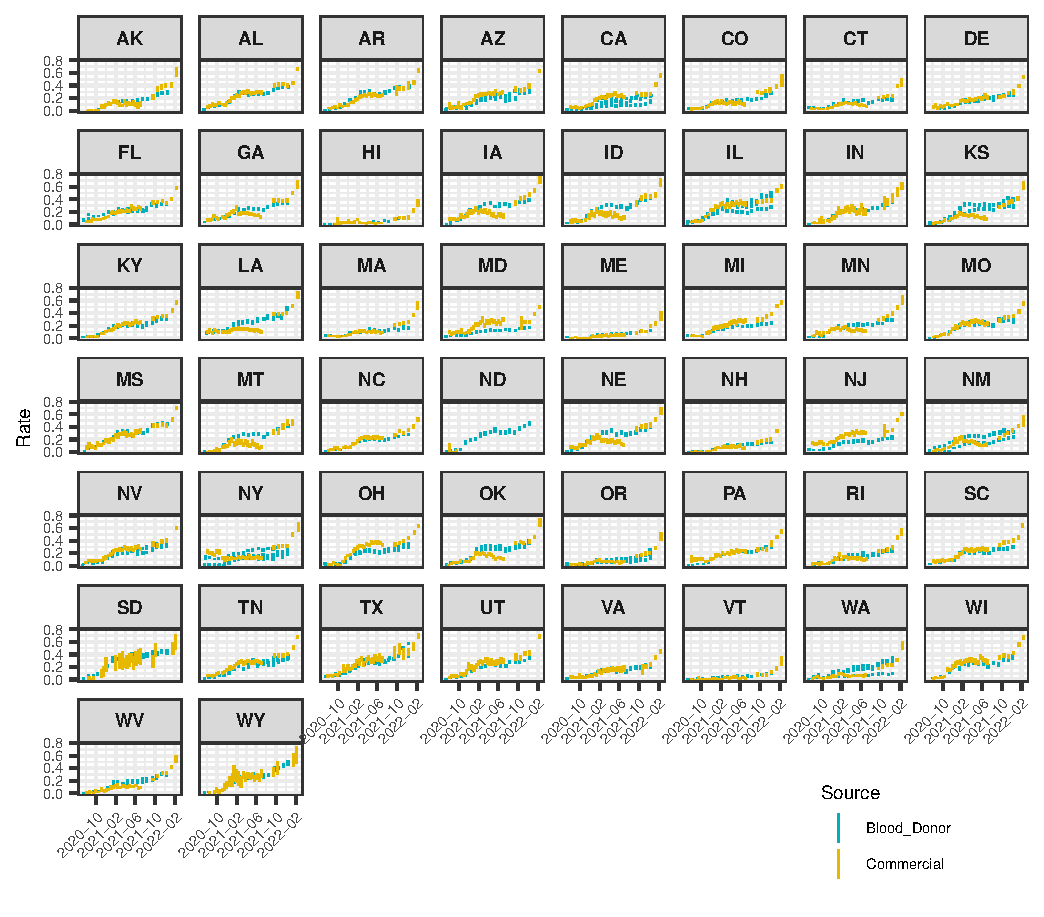
\includegraphics[width=.99\textwidth]{sero_blood_comm_compar.pdf}
    \caption{A comparison of the seroprevalence estimates from the Commercial
    Lab Seroprevalence Survey dataset (yellow) and the 2020--2021 Blood Donor 
    Seroprevalence Survey dataset (blue). Note that the maximum and the minimum
    of the line ranges are the provided 95\% confidence interval bounds to 
    give a rough indication of uncertainty.}
    \label{fig:sero_blood_comm_compar}
\end{figure}

The date variables that come with the two seroprevalence datasets are different
and so the date variables that we are able to construct from them are
not the same. For the commercial dataset, we use the midpoint of the provided
specimen collection date variable. A major difference in the structure of the
two datasets is that the commercial dataset always has the seroprevalence
estimates at the level of the state, while the blood donor dataset can either have 
estimates for the state or for multiple separate regions within the state. For the 
blood donor dataset, we use the median donation date if the seroprevalence 
estimates are designated to be for entire state. If they are instead for regions in 
the state, since there is reliably one measurement per region per month, we 
aggregate the measurements into one per month per state by using a weighted 
average (to account for the given sample sizes of the regions). The median of the 
median dates is taken to be the date for the weighted average.

For adjusting our infection counts, annual estimates of the resident state
populations as of July 1 of 2020 and 2021 are taken from the December
2022 press release on the \US\ Census Bureau website \citep{uscensus2022annual}.
Unless otherwise specified, we use the July 1, 2020 estimates.

The daily fraction of new infections are estimated from the provided incidence
of suspected reinfections over March 2020 to April 2022 in Clark County, which
is based on surveillance work conducted by the Southern Nevada Health District
(SNHD) and reported by \citet{ruff2022rapid}. The proportion of new cases per
week that are suspected reinfections are calculated by dividing the number of
suspected reinfections by all new PCR-identified cases during the same week. 
%Possible problem here – reinfections not include third infections (see comments
% in the discussion section about this)

% Possible change to the paper based on Ajitesh's feedback - 
% Main contribution is the model, shows without reinfection 
% & here's an extension that shows how to include reinfection data. 

\subsection{Estimating the delay from positive specimen to report date} 

We use the restricted CDC line list to estimate the distribution between positive specimen
 and report for each state at each time. To formalize this, let
$y_t$ denote the count of new cases reported at time $t$ and $x_t$ denote the
count of deconvolved cases with positive specimen at $t$. 
For all cases in the line list that had both a positive specimen and a report date, 
we can count the those that are
reported at time $t$ by enumerating them according to positive specimen date 
(similar to how symptom onset date was used in \citealp{jahja2022real}):
\begin{align*}
y_t = \sum_{s=1}^{t} \sum_{i=1}^{x_s}\indicator \left ( \text{the }i\th\text{ positive specimen at }
 s \text{ gets reported at }t \right ).
\end{align*}
Taking the conditional expectation of the above yields
\begin{align*}
\E(y_t \mid x_s, s \leq t) = \sum_{s=1}^{t} \pi_t(s) x_s ,
\end{align*}
where $\pi_t(s) = \P(\text{case report at }t \mid \text{positive specimen date at }s)$ for
each $s \leq t$ are the delay probabilities and the $\{ \pi_t(s) : s \leq t
\}$ sequence comprises the delay distribution at time $t$. Notice that
there are no time restrictions placed on the positive specimen date, except that it must
have been between the start of the pandemic and the report date, inclusive. This is
unlikely to be a realistic assumption to make as $t$ moves farther away from
$s$. 

Thus, we make two key assumptions about these distributions. First,
positive specimen tests that are reported to the CDC are always reported within $d = 60$
days, which is true for the majority of the reported cases. Second, the
probability of zero delay is zero, which stems from the contamination of
zero-delay in the line list. As in \citet{jahja2022real}, we update the
conditional expectation formula to reflect these two assumptions: 
\begin{align*}
\E(y_t \mid x_s, s \leq t) = \sum_{k=1}^{60} p_t(k) x_{t-k}
\end{align*}
where for $k = 1, \dots, 60$,
\begin{align*}
p_t(k) = \P(\text{case report at }t \mid \text{positive specimen at }t-k).
\end{align*}

For each state, we estimate the positive specimen to report date distribution
 at each $t$ by using the empirical distribution of
all non-zero lags between the complete cases whose positive specimen dates fall in the
 interval around $t$ designated by $[ t - 75 + 1, t + 60]$). 

Now, the task of estimating the positive specimen to report date distribution
 for each state at each time requires four distinct steps. First, we obtain the empirical
distribution of all lags (excluding zero) from all cases with positive specimen dates
falling in the roughly center-aligned interval. Next, we weight the state-specific
empirical distribution by the proportion of CDC cases to JHU cases. That is, we
compare the number of CDC cases used to create the empirical distribution to the
number of cases reported by JHU in the time window of $\left[t - 60 + 2, t +
75\right]$ (to correspond appropriately to the interval for
the CDC cases). This proportion is used as the weight for the state's empirical
distribution, while the complement is used to weight the overall empirical
distribution that is formed from the data for all states. This construction
allows for more reliance on the state's distribution when there are more CDC
cases relative to JHU (and vice versa). After implementing the shrinkage method,
we fit a gamma density to the resulting empirical distribution by the method of
moments. Finally, we discretize the resulting density to the support set of 1
to 60 days.
 
\subsection{Estimating the delay from symptom onset to positive specimen date}  \label{delaystop} %% Maybe add appendix plots here?

The task of estimating the delay from symptom onset to positive specimen date 
follows the same procedure as for positive specimen to report date with a few key
 data-driven amendments. Firstly, we allow for negative delays to account for the
  possibility that an individual case tests positive before symptom onset. Under this
   assumption, the lower and upper bounds for the support of $-3$ and $21$ are 
   chosen based on the largest delay values for the statewise 0.05 and 0.95 quantiles
    that are not outliers. Secondly, we allow for zero delay because the median 
    statewise delay is very short at approximately 2 days. Thirdly, there are times where
     the empirical probability was observed to be precisely 1 at zero delay and the 
     proportion of CDC relative to JHU cases used for the weight was also 1. Since 
     we believe that having zero delay for all cases is unrealistic and unlikely to be 
     representative of all cases for the state, we inject a small amount of variance 
     manually by setting the the CDC-to-JHU proportion to be the minimum shrinkage
      proportion observed for the affected state (such instances were isolated to the
       state of New Hampshire). Aside from these modifications, the construction of 
       the delay distribution proceeds in precisely the same manner as for positive 
       specimen to report date. 

\subsection{Estimating the incubation period distributions} 

One incubation period distribution is estimated for each variant under consideration.
The variants we consider are Alpha, Beta, Gamma, and Delta, which are
 included because they are
are designated to be variants of concern by WHO based on their potential to
cause new waves, dethrone the dominant variant, and lead to changes in public
health policy \citep{who2021tracking}. In addition, we include the Epsilon
(California) and Iota (New York) variants because of their impact on those and
the surrounding states \citep{yang2022investigation, duerr2021dominance}. We
relegate all other variants to be in the Other category (which, for our purposes,
is treated as a catch-all for all 2020 Ancestral variants observed in the U.S.)
This decision to include an Other category is, in part,
motivated by the lack of sequencing data for most states in 2020 as well as the
presence of an Others category in the sequencing data for that time. 

We construct the incubation period distributions for the variants as gamma distributions.
These distributions are the same for all states and based on literature estimates of the gamma 
parameters or the
mean and standard deviation of the incubation period (in which case the method
of moments is used to fit a gamma density). Then, we discretize each
resulting density to the support set, which is taken to be from 1 and
21 days. In other words, those are taken to be the lower and upper limits for
the number of days that the virus could be incubating in someone. The implicit
assumption for the lower bound is that there must be at least one day between
infection and symptom onset (which follows the convention given in
\citealp{phcan2021covid}). The assumption underlying the upper bound is that 21
days is the maximum number of days that the virus could be incubating in someone
(which is reasonable based on \citealp{zaki2021estimations} and
\citealp{cortes2022sars}).

\subsection{Convolutional estimates of the infection to positive specimen distributions} 

The previous two steps enabled us to estimate one incubation period per variant
and one symptom onset to positive specimen distribution for each state at each time under
consideration. We proceed to convolve each such pair of distributions to get estimated
infection to positive specimen distributions and, hence, estimated time-varying probabilities for
the delay from infection onset to positive test specimen date for each state.

\subsection{Retrospective deconvolution}

The main goal for the retrospective deconvolution stage is to estimate the daily number of new
infections for each time using the dates that those cases were eventually
reported. To this end, there are two types of deconvolution performed. The first is the 
deconvolution from report to positive specimen date and the second is from positive specimen
 date to infection onset date. We allocated the deconvolutions in this way to allow us to get
  the daily deconvolved case estimates by variant. The intermediate of positive specimen
   date was chosen because the variant proportion estimates are aligned to this date. 
   So for each state at each time, nine deconvolutions are performed in total. 
   The first is the deconvolution from report to positive specimen date, 
   followed by the eight deconvolutions from positive specimen to infection onset for
    the eight different variant categories.

We will start by describing the first type of deconvolution performed from
 report to positive specimen date in detail and
then describe the second type in terms of the changes made with respect to the first.
For each state, we achieve the first goal to estimate positive specimen dates for the
 cases by solving an optimization problem. 
% Following the notation of \citet{jahja2022real} (save for suppressing the
% state/location subscript), 
For this problem, let $\cT$ represent the extended deconvolution period from March 1, 2020 to 
March 1, 2023, which was used to minimize the effect of boundary issues and to produce
 sufficient deconvolved case estimates for further analysis.
Let $\hat{p}_t$ be probabilities from the estimated
positive specimen to report date distribution for $t \in \cT$, $y_t$ the number of new cases
reported, and where $D^{(4)}$ is the discrete derivative matrix of order 4
such that $D^{(4)}x$ yields all $4\th$-order differences of the vector $x$. From these,
we estimate the deconvolved case counts across time by solving for the vector $x$ in
\begin{align*}
\minimize_{x}\ \sum_{t \in \cT} \left ( y_t -  \sum_{k = 1}^{d} \hat{p}_t(k)x_{t-k} 
\right )^2 + \lambda \|D^{(4)}x\|_1. 
\end{align*}

The above loss function decouples into two parts which trade data fidelity with
desired smoothness (that
encapsulate the classic bias-variance trade off). The first part represents
minimizing the sum of squared errors between the JHU reported cases and the
estimates, while the second part captures the smoothness of the estimates
(smaller values being more smooth). The tuning parameter $\lambda$ determines
the relative importance of these competing goals.

We solve this trend-filtering-regularized least squares deconvolution problem by
employing the ADMM algorithm from \citet{ramdas2016fast} that is described in
Appendix A of \citet{jahja2022real}. The solution to the problem is an adaptive
piecewise cubic polynomial \citep{tibshirani2014adaptive,
tibshirani2022divided}.

We select the tuning parameter, $\lambda$, by using $3$-fold cross validation similar to
\citet{jahja2022real} in which every third infection count is
reserved for testing. The tuning parameter that results in the smallest mean
 squared error is selected.

From this first type of deconvolution, we obtain case estimates by positive
 specimen date for each state.
The second type of deconvolution, where the goal is to get estimates of the
 infection onset date for these cases, follows the form of first type, save for two
  key modifications to the inputs. Firstly, we utilize the results from the first deconvolution
   and, secondly, we must update the probabilities to be the convolutional estimates 
   of the infection to positive specimen distributions. Thus, for a fixed variant category, 
   $y_t$ is the number of new cases deconvolved to positive specimen date multiplied 
   by the estimated proportion of the variant in circulation in the state at $t$, and $\hat{p}_t$
    are the probabilities from the estimated infection onset to positive specimen distribution
     for $t \in \cT$. With these modifications to the inputs, the deconvolution proceeds in the
      exact same way as before. Since this deconvolution is done separately for each variant
       category, we ultimately obtain deconvolved case estimates by the date of infection onset 
       that are separated by variant.

\subsection{Inverse reporting ratio and the antibody prevalence model} 

The infection estimates from retrospective deconvolution are
derived solely from the infection onset dates of the reported cases. 
To capture the unreported infections, it is necessary to adjust these
deconvolved case estimates by 
a scaling factor that approximates the ratio of the true number of new infections
to the new reported infections. We refer to this quantity as the
inverse reporting ratio and denote it by $a_t$ for day $t$. Our new goal is
to estimate this quantity for every state at every time under consideration from
June 1, 2020 to November 29, 2021.

The number of new reported infections is obtained from our
deconvolved case estimates. As for the true
infections, since seroprevalence of anti-nucleocapsid antibodies is used to
estimate the percentage of people who have at least one resolving or past
infection \citep{cdc2020data}, we can use
the change in subsequent seroprevalence measurements to capture new infections, 
accounting for those whose antibody levels fall below the detection threshold.
We can adjust the retrospective deconvolution estimates using a model that is 
based on such seroprevalence estimates.
 
To adapt to the sparseness in the seroprevalence data, we convert our daily data 
to weekly by summing the reported infections and shifting the observed 
seroprevalence measurements to the nearest Monday. If there are multiple 
measurements in a week from a seroprevalence source, then the average is used. 
We denote these changes by changing the time-based subscript 
from $t$ to $m$ where $m$ indicates the Monday 
relative to our June 1, 2020 start date.

For each state, let $s_m$ be the seroprevalence estimate on $m$, $w_m$ be the
corresponding inverse variance weight, and
 $C_{m-1}^m = \sum_{t = m-1}^{m} c_t$ be the total reported infections from $m-1$ to $m$
scaled by the state's population. 
To account for reinfections, we multiply the change in reported infections for $m$
by the corresponding fraction of new infections, $z_m$. 

Using these components, we construct the following model separately for each state
%\begin{align}
%\min_{a, \gamma}\frac{1}{2}\sum_{t \in T}w_t\left (s_t - (1 -\gamma)s_{t-1} 
%- a_t \Delta C_t z_t  \right )^2 + \frac{\lambda}{2} \|D^{(3)}a\|_2^2 \label{eq:waningpr}
%\end{align}
%  $w_t$ be the inverse variance weights derived from those estimates,
\begin{align}
s_m &= (1 -\gamma)s_{m-1} + a_m C_{m-1}^m z_m + \epsilon_m, \qquad \epsilon_m \sim N(0, w_m \sigma^2_\epsilon) \label{eq:waningpr}  \\
a_{m+1} &= 3a_{m} - 3a_{m-1} + a_{m-2} + \eta_m,\qquad\qquad \eta_m \sim N(0, \sigma^2_{\eta})   \nonumber
\end{align}
where $\gamma$ is the percentage
of people whose level of infection-induced antibodies falls below the detection 
threshold between time $m$ and time $m+1$.
Informally, we refer to $\gamma$ as the waning parameter and we call this model the population 
antibody prevalence model. 
% By ``waning'' we are referring to the natural decline in the infection-induced antibodies over time. 
%Since the true course of immunity over time is unknown
% \citep{goldberg2022protection}, we take the straightforward approach 
% and model one $\gamma$ to try avoid making gratuitous
% or overly restrictive assumptions. 

We express the antibody prevalence model as a state-space model. This representation
allows for convenient handling of missing data, extrapolation before and after
the period of observed seroprevalence measurements, and maximum likelihood
estimates of $\gamma$ and $\sigma^2_\epsilon$. Details of this methodology and
the computation of the associated uncertainty measurements are deferred to the
Supplementary Materials \ref{supp:ssapm}.


\subsection{Lagged correlation to hospitalizations and time-varying IHRs} 

We use our infection estimates in a lagged correlation analysis with
confirmed COVID-19 hospitalizations. Our primary goal of this analysis is to
find the lag between infection and hospitalization rates that gives the highest
average rank-based correlation across \US\ states. To that end, we consider a wide
range of possible lag values ranging from 1 to 25 days. Zero and negative
lags are not considered because COVID-19 infection onset must precede
hospitalization due to the virus. To remove day of the week effects, both the
infection and hospitalization signals are subject to a 7-day moving
average (center-aligned) before their conversion to rates.

For each considered lag, we calculate the Spearman's correlation between the 
state infection and hospitalization rates for each observed day 
over the June 1, 2020 to November 29, 2021
time period %, and use the epi\_slide function \citep{mcdonald2023epipredict} to 
with a center-aligned rolling window of 61 days for each such computation.
We then calculate the average correlation across all states and times for each lag. 
The lag that leads to the highest average correlation is used to estimate 
the time-varying IHRs for each
state. To compute this for a given day, the number of individuals who are
hospitalized due to COVID-19 on a day are divided by the estimated total number
who were infected on the lagged number of days before.

\subsection{Ablation study for the lagged correlation analysis} 

To better understand the contribution of the intermediate steps to the lagged 
correlation analysis, we carry out a brief ablation study in which we calculate the 
lagged correlation using the following infection estimates: 1. those from the
deconvolution procedure under the assumption that the infection onset is the
same as the positive specimen date 
(i.e., excluding the positive specimen to infection onset data and deconvolution); 
2. those from the deconvolution procedure under the assumption that the infection onset is the
same as the symptom onset date (excluding the incubation period data); 
3. those from the deconvolution procedure when utilizing all incubation period and delay data 
(the deconvolved case estimates); 4. those from applying the antibody prevalence 
model to produce estimates for both the reported and the unreported 
cases (the infection estimates).

\section{Results}

This work estimates incident infections for each \US\ state over June 1,
2020 to November 29, 2021 and to illustrate the disease burden and viral
transmission dynamics at the level of the state across time. After converting the number
of infections to rates (infections per 100,000 population), we perform a
brief comparison between infection and case estimates within each state to see
to what extent that surges in infections are evident in cases alone
and point out instances where cases largely fail to capture surges in infections.
To apply these infection estimates, we perform a lagged correlation analysis
with hospitalizations and then compute the time-varying IHRs for each state.
Finally, we look at infections within and across the states and point out patterns related
 to the major variants and geographical contiguity.
% postulate what may be 
% contributing to these trends based on defining characteristics such as geographical contiguity.  

\subsection{Infection estimates compared to reported cases}

Naturally, outbreaks in infections precipitate those in cases and are reliably larger in
magnitude (\autoref{fig:state_infect_est}).
Hence, our infection estimates indicate
that the pandemic had a differential impact across states earlier and at a larger scale
than is suggested by cases. From the choropleth maps that compare the state-level rates 
of daily new infections and cases per $100,000$, we can observe
that for the earliest time of June 1, 2020, there is little discrepancy between case
and infection rates, while for the later times there are immense differences in the
rates, such that case rates tend to underrepresent infections to a great extent 
(\autoref{fig:choro_inf_case_rates}).

While the major Ancestral, Alpha, and Delta waves tend to be
visible for most states, there are clear outbreaks in unreported infections 
that are not easily detectable from cases alone in the 
falls of 2020 and 2021. For example, take the wave in the spring of 2021 for North Dakota and
South Dakota, where the relatively flat and steady case cadence fails to capture the major 
wave of infections. With respect to variants of concern, consider the late 2020 Ancestral 
wave for the midwestern states of Illinois, Indiana, and Ohio. For the major Delta wave, some
 of the greatest discrepancies between cases and infections are visible in the western states 
 of Idaho and Montana, the southern states of Louisiana and Georgia, and the midwestern 
 states of Iowa and Nebraska (\autoref{fig:state_infect_est}). Earlier on in the pandemic, such 
 discrepancies between cases and infections may be more attributable to failures in the reporting 
 pipeline, while later on in the pandemic, they more likely due to the rise in asymptomatic infections
across variants \citep{oph2022covid, garrett2022high}. 

Finally, while the main Delta wave is somewhat evident from the case counts for all states 
(\autoref{fig:state_infect_est}), our estimates suggest that case counts tend to severely 
underestimate infections during this time for many states. The lowest of all states was in New Jersey,
where about $4.6\%$ (95\% confidence interval: $[1.9, 67.7]$) of the estimated infections were
 reported. This was followed by Maryland with $7.4\%$ ($[2.7, 83.8]$), Connecticut
with $8.0\%$ ($[3.1, 25.8]$), and Florida with $8.7\%$ ($[4.8, 34.0]$). This underreporting 
issue extends to most states as in $39$ states less than $30\%$ of infections were reported during
 this time. Only $4$ states of Alaska, Maine, Vermont and Virginia reported at least $40\%$ infections. 
 No states were found to surpass $50\%$ for reported infections for this time.

Similar patterns were observed during the earlier period of Alpha domination, 
where Louisiana had the lowest reported infections at 
$11.7\%$ (95\% confidence interval: $[6.7, 31.5]$) and was followed by California at 
$14.4\%$ (95\% confidence interval: $[7.7, 68.2]$). There were $23$ states that reported at least 
$40\%$ and $22$ states that reported at least $50\%$ of their infections.

Such patterns were comparatively less apparent during the earlier and larger period of Ancestral
 domination, where Ohio and Maryland held the lowest percentages of reported infections at 
 $22.0\%$ (95\% confidence interval: $[16.2, 34.0]$) and $22.3\%$ 
 (95\% confidence interval: $[14.8, 40.5]$), respectively. During this time, $28$ states
  that reported at least $40\%$ and $14$ states that reported at least $50\%$ of their infections. 

\autoref{fig:six_state_est} zooms in on the infection estimates for the states that exhibit the most
 underreporting for each of the three variant-specific time periods to emphasize the marked differences
  between case and infection rates. To supplement this, \autoref{fig:six_state_decon_byvar_est} 
  shows the division of infections in states by the proportions of variants in 
  circulation specific to the state. From these plots, it is clear that few variant categories tends
   to dominate and drive infections at a time. The general progression in terms of variant starts
    with the Ancestral category from 2020 up to early 2021, 
to the Alpha variant in mid 2021, which eventually gets eclipsed by the Delta variant in mid to late 2021. 
This supports our division of our results by the three main variant-driven time periods.

\begin{landscape}
\thispagestyle{empty}
\begin{figure}[!tb]
    \centering
    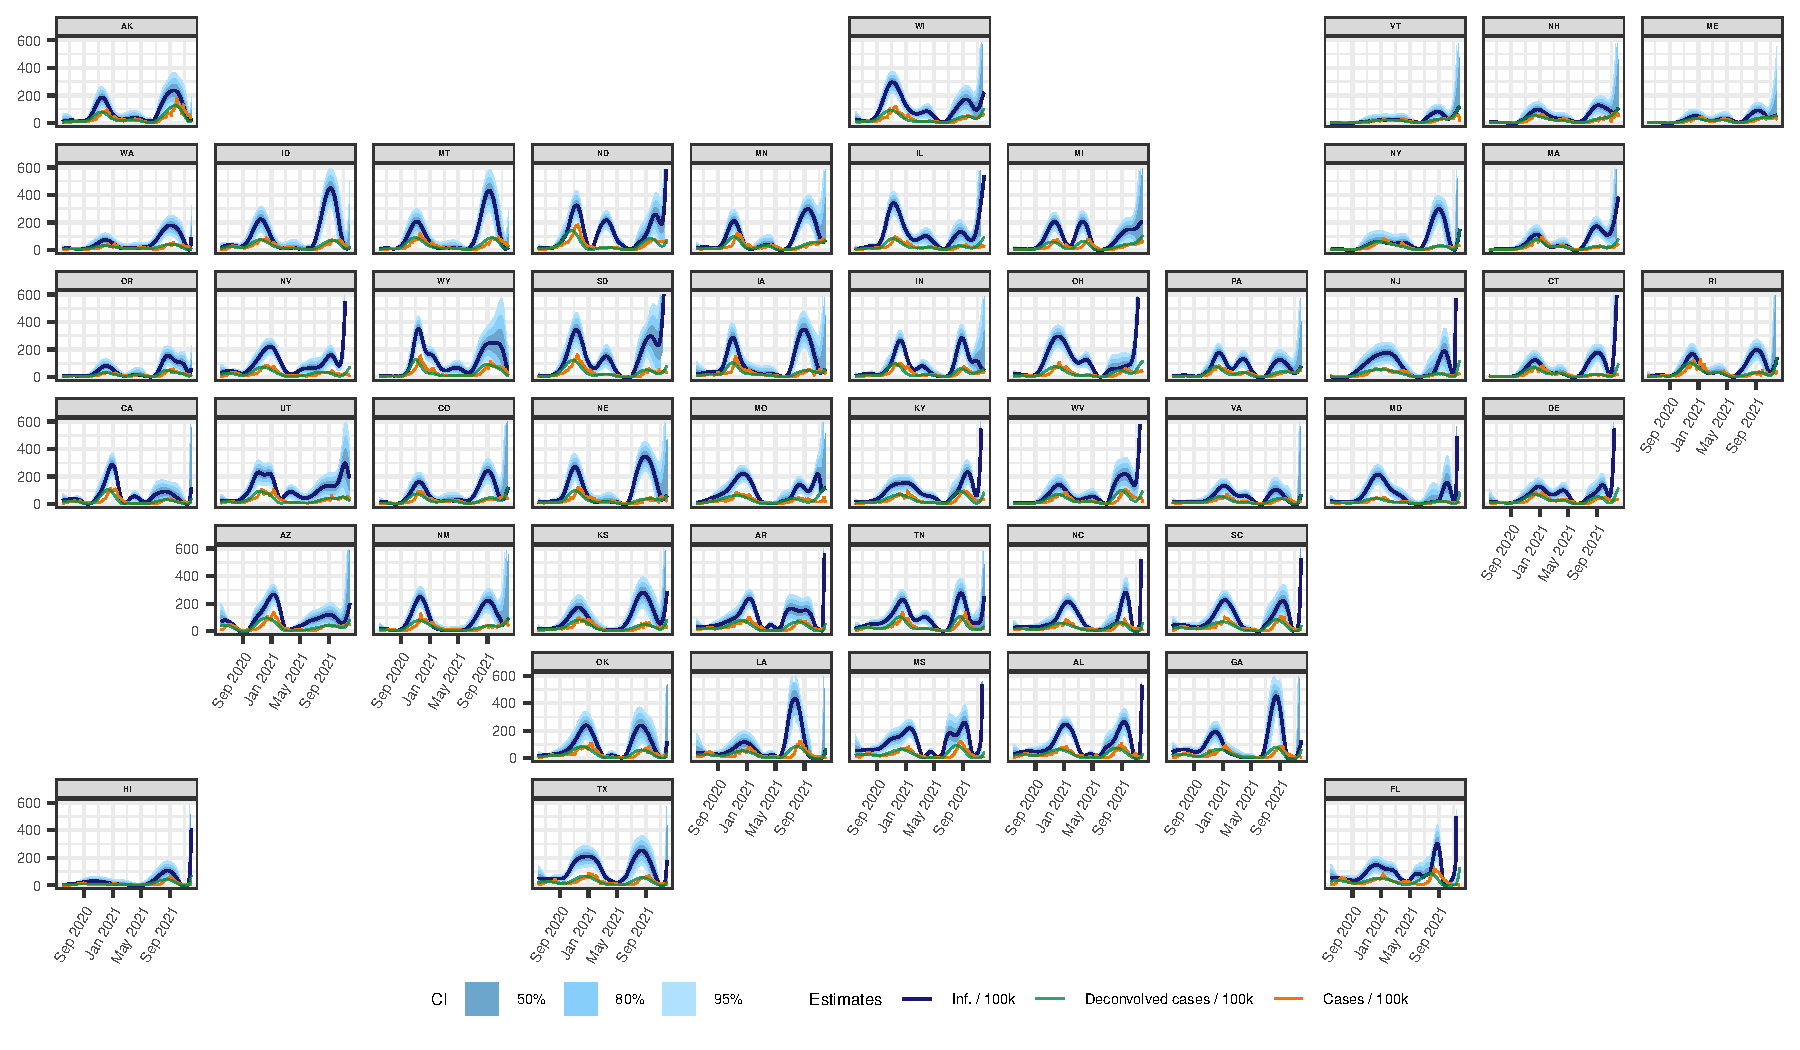
\includegraphics[width=.99\linewidth]{state_niauc_est_faceted_F24.pdf} 
    \caption{Estimates of the number of daily new infections per
     100,000 population for each \US\ state from June 1, 2020 to November 29, 2021
      (dark blue line). The blue shaded regions depict the 50, 80, and 95\% confidence 
      intervals for the estimates, while the teal line represents the 
      number of new daily new deconvolved cases per 100,000, and the dotted 
      orange line represents the 7-day average of the new cases per 100,000 as 
      of the same date.}
    \label{fig:state_infect_est}
\fillandplacepagenumber
\end{figure}
\end{landscape}

\begin{figure}[!tb]
\centering
    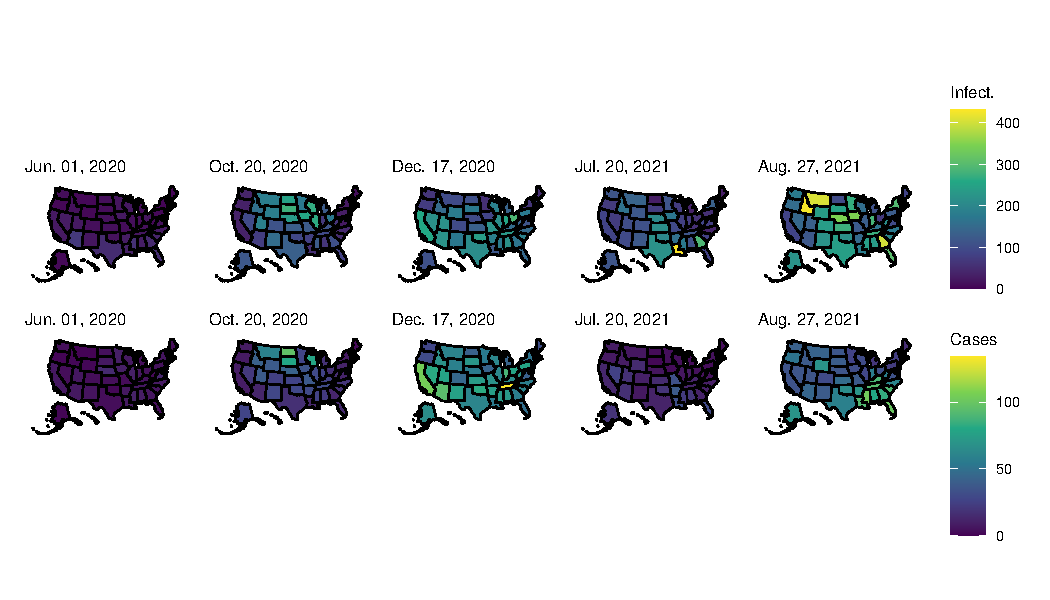
\includegraphics[width=.99\textwidth]{choro_inf_case_rates_F24.pdf}
    \caption{Choropleth maps of the state-level estimates of the number of 
    daily new infections per $100,000$ population (top row) and the 
    daily new cases per $100,000$ population (bottom row) for three times
    over the June 1, 2020 to November 29, 2021 period. The first date was
     chosen simply as a baseline, while the second and third 
    dates were chosen based on the day that had the largest number of infections 
    across the 50 states from each year. 
    These maps are generated from the \texttt{usmap} 
    package in R \citep{lorenzo2023usmap}.} 
    \label{fig:choro_inf_case_rates}
\end{figure}

\begin{figure}[!tb]
\centering
    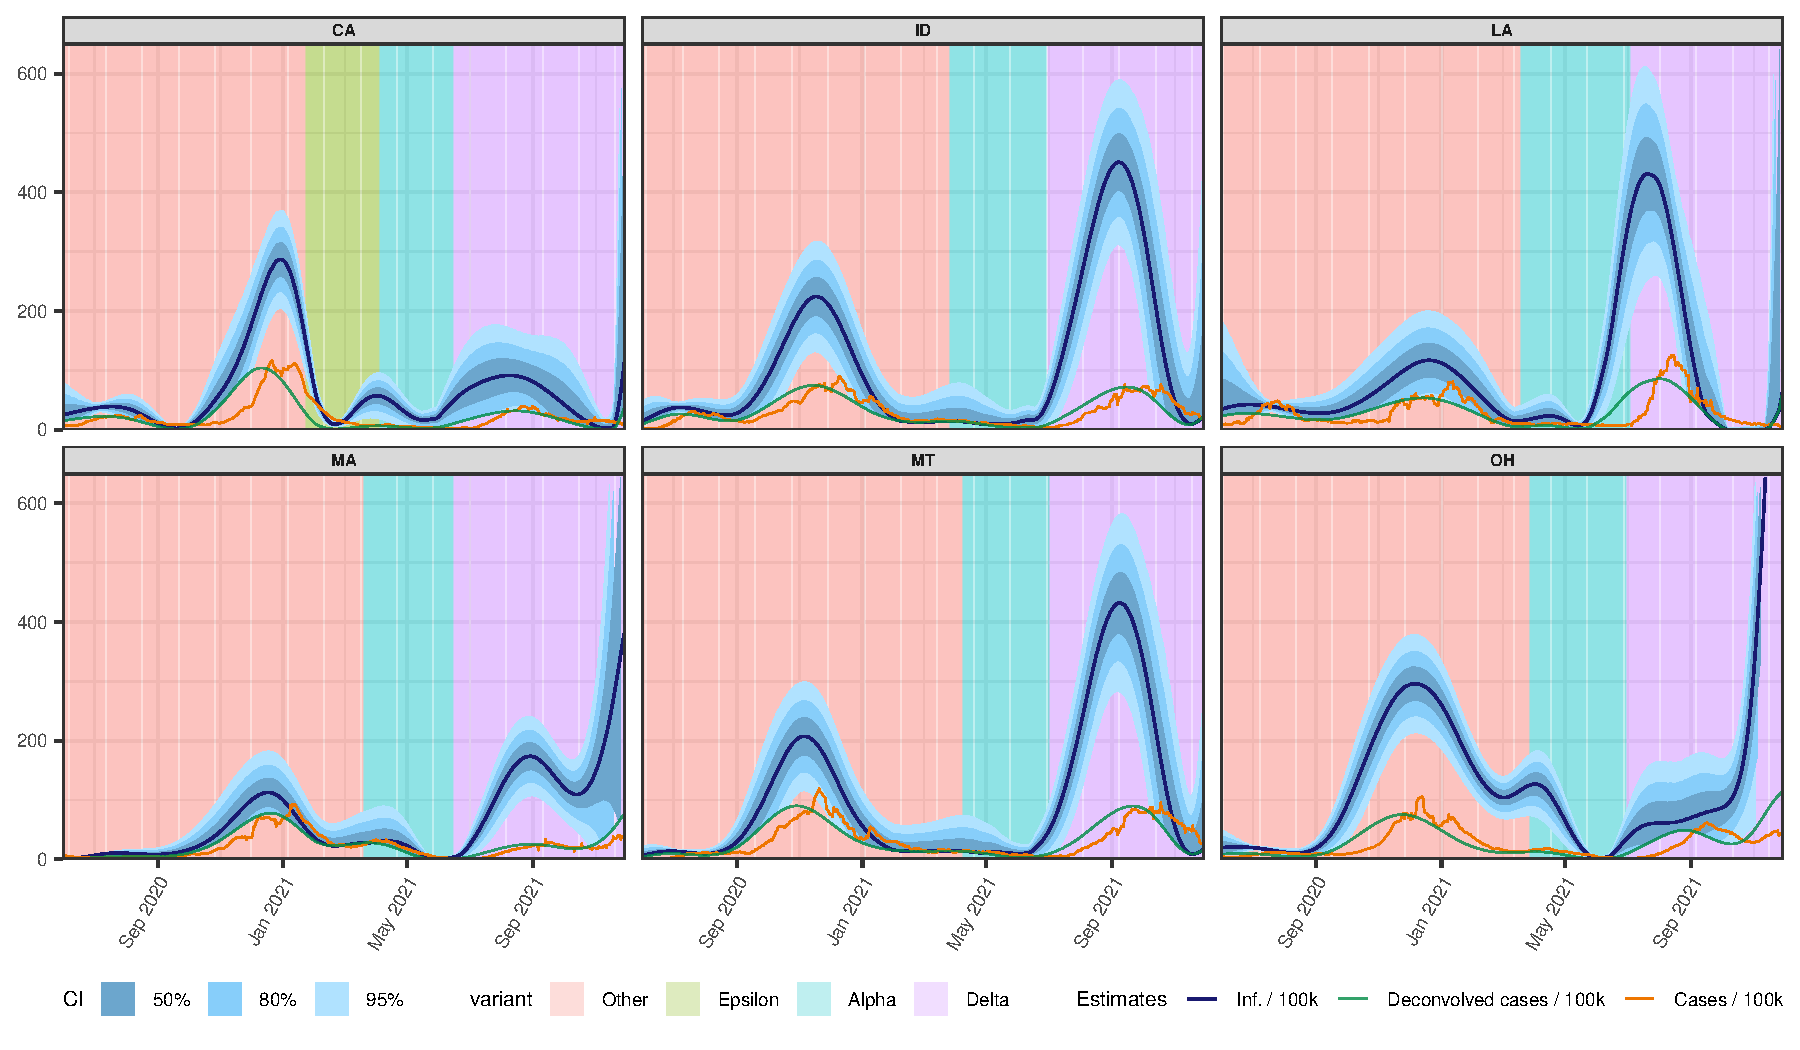
\includegraphics[width=.9\linewidth]{state_niauc_est_6states_F24.pdf}
    \caption{Estimates of the number of daily new infections per 100,000 for
    six \US\ states from June 1, 2020 to November 29, 2021 (dark blue
    line). The blue shaded regions depict the 50, 80, and 95\% confidence
    intervals. The background is shaded to indicate the top variant in
    circulation at the time.}
    \label{fig:six_state_est}
\end{figure}


\begin{figure}[!tb]
\centering
    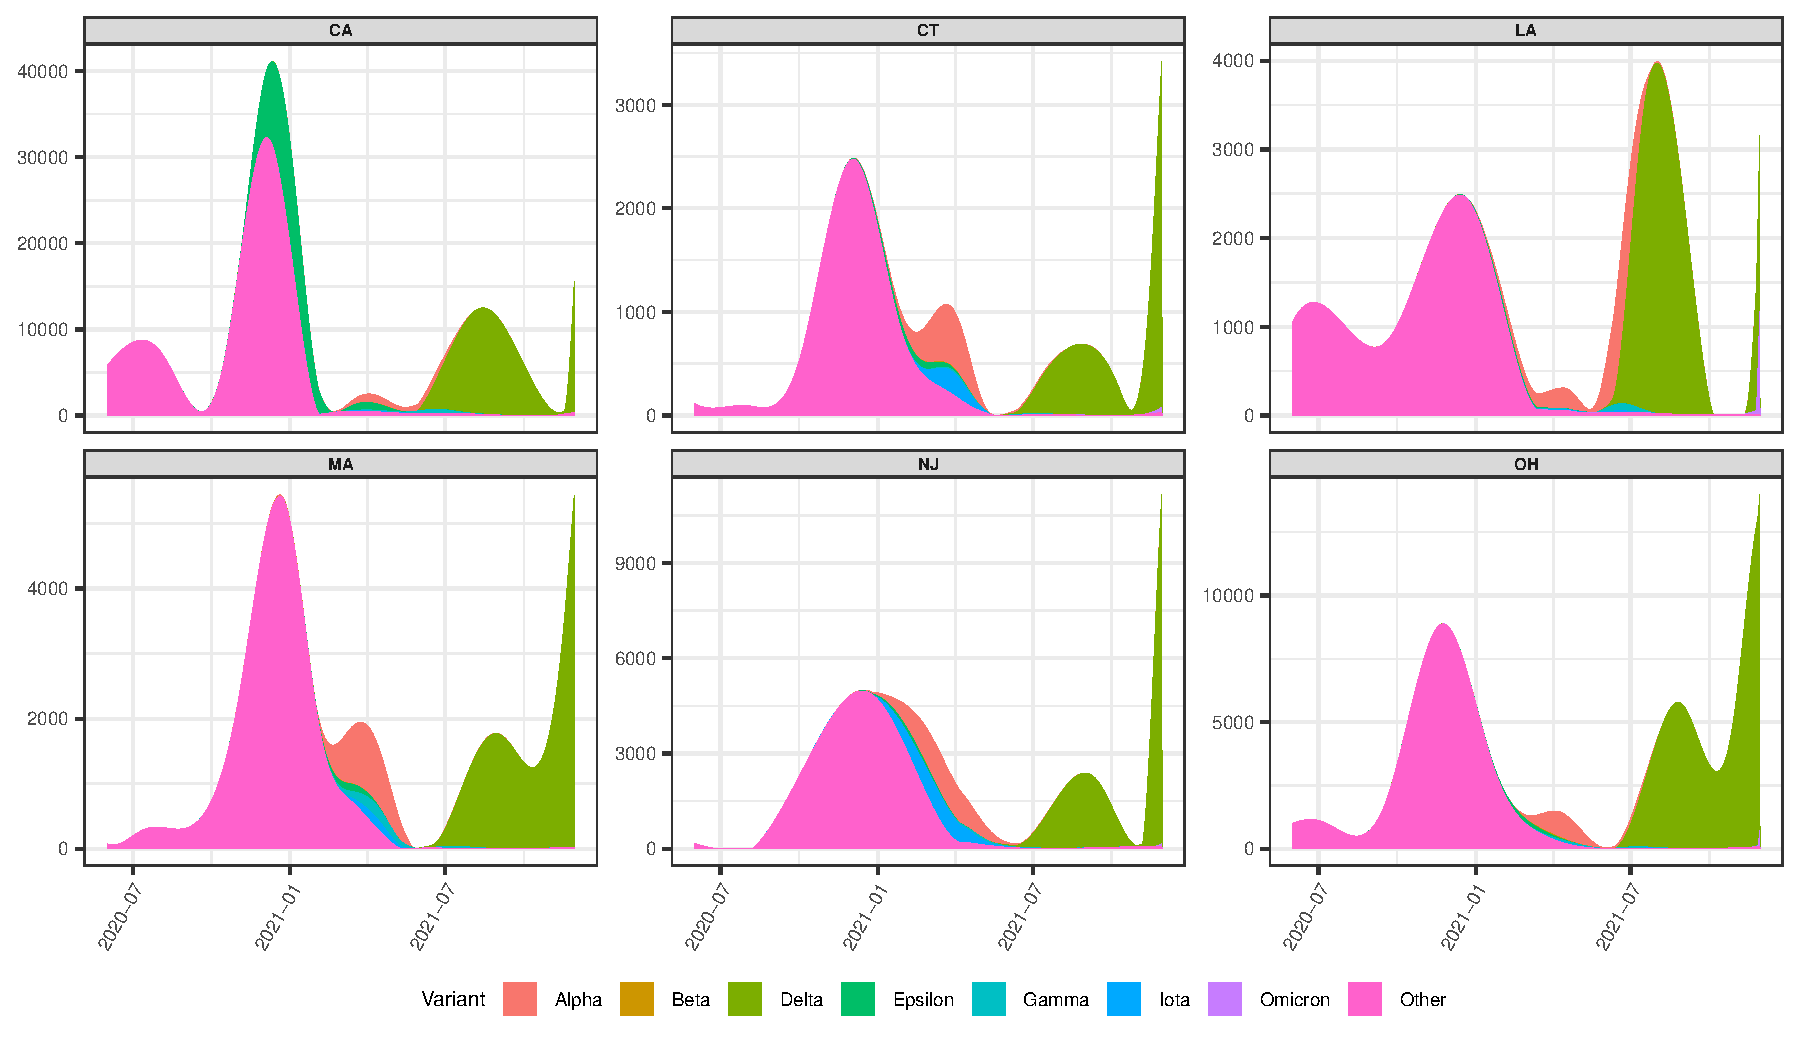
\includegraphics[width=.9\linewidth]{state_decon_byvar_est_6states_F24.pdf}
    \caption{Estimates of the deconvolved case counts by variant for
    six \US\ states from June 1, 2020 to November 29, 2021. 
    The area under the curve is coloured to indicate the corresponding variant.}
    \label{fig:six_state_decon_byvar_est}
\end{figure}

We perform a lagged correlation analysis where we systematically investigate the
rank-based (i.e., Spearman's) correlation between our infection and confirmed
hospitalization rates per 100,000 population over a broad range of lag values
(\autoref{fig:infect_case_hosp_lag_corr}). Examining the correlation between infections and
hospitalizations shows that the maximum average correlation across states of $0.513$ is 
first observed at a lag of $13$ days. In contrast, we find that the greatest average
rank-based correlation for cases of $0.691$ is achieved at a lag of 
$1$ day. That is, we find that case report rates are nearly contemporaneous to 
hospitalizations, while infection estimates clearly precede them. 

We undertake an ablation study for the lagged correlation of infections, the results of which 
are shown in \autoref{fig:adj_unadj_sym_hosp_lag_corr}. From this, we can see that the 
deconvolved case or infection estimates from the intermediate 
steps are all leading indicators of hospitalizations. However, the degree that each such set of estimates
lead hospitalizations depend on its location in the sequence of steps and how close the estimates 
are to infection onset. For example, the deconvolved cases by positive specimen date
tend to precede hospitalizations by about $11$ days, 
while those for the subsequent step indicate that the deconvolved cases by symptom onset tend to 
precede hospitalizations by a longer time of about $13$ days. Finally, after adding the variant-specific 
incubation period data into the deconvolution and obtaining the deconvolved case estimates, 
we can observe that the reported infections precede
hospitalizations by about $17$ days. 

In terms of the average correlation produced, the deconvolved case estimates by infection onset
 and the deconvolved case estimates by positive specimen date reach almost
  the same maximum average correlation. While that is not a clear differentiator by itself, 
  there is a clear time-based benefit of opting for the infection estimates by the date of infection onset
   over symptom onset because they provide similar information 
on hospitalizations about $6$ days before the latter tends to occur.

Unsurprisingly, the deconvolved case and infection estimates achieve their maximum correlation
at the same lag. And yet, the average correlation to hospitalizations
tends to be greater for the deconvolved case estimates than for the infection estimates (and
the reported infections by symptom onset). If the goal is to find the part of this process that is most
 informative to hospitalizations, then it is clear that producing the deconvolved case estimates is 
 the more informative step and these estimates are potentially the most meaningful signal for
  future hospitalizations. The reason for this finding may stem from a difference in disease
   severity between the reported and unreported infections: The unreported infections tend to 
   be less severe and less likely to lead to hospitalization than those that are reported.

As a counterpart to our lagged correlation analysis, we compute the time-varying IHRs 
for each state using the optimal lag for infection and hospitalization rates. We also included
the CHRs that are computed using the optimal lag for cases and hospitalizations for comparison
(\autoref{fig:IHR_7dav}). 

For each state, the CHRs tend to show an amplified version of the course of the IHRs over time.
This supports our claim that the reported infections are more likely to require hospitalization
than the unreported infections. Both the IHRs and CHRs exhibit similar geospatial and 
temporal trends as are noted for infections. 
Namely, states that are close in proximity (such as Ohio, Pennsylvania, and Virginia) tend to 
exhibit similar patterns in the IHRs and CHRs over time. In addition, 
there are similar spikes observed across many states during 
waves of infections that are driven by prominent new variants. For example, many
states exhibit a striking spike in hospitalizations in mid-2021, which coincides with the rapid takeover 
of the Delta variant during that time \citep{hodcroft2021covariants}. This finding aligns with 
previous studies that found an increased risk in hospitalizations with Delta in comparison to other
variants \citep{twohig2022hospital, nyberg2022comparative}. Similarly, during the fall of 2020 
there tends to be another spike in the IHRs
that rivals or surpasses that observed during the time of Delta (which is the case for states
 like New York or Wyoming). 

There does not tend to be a strict upwards or downwards trajectory or even a mild waning pattern
 in the IHRSs (as one might expect if we were to tread further into the pandemic over
  which the virus mutates to variants that are generally more infectious, but that
   pose less of a risk to hospitalization \citep{lorenzo2022covid, blauer2022compare}). 
Overall, we observe intermittent spikes that punctuate longer periods where the IHRs 
tend to be less than $0.2$ hospitalizations per infection. 
These spikes tend to align with the emergence of new variants.  % and seasonal changes.

\clearpage
\begin{figure}[!tb]
\centering
    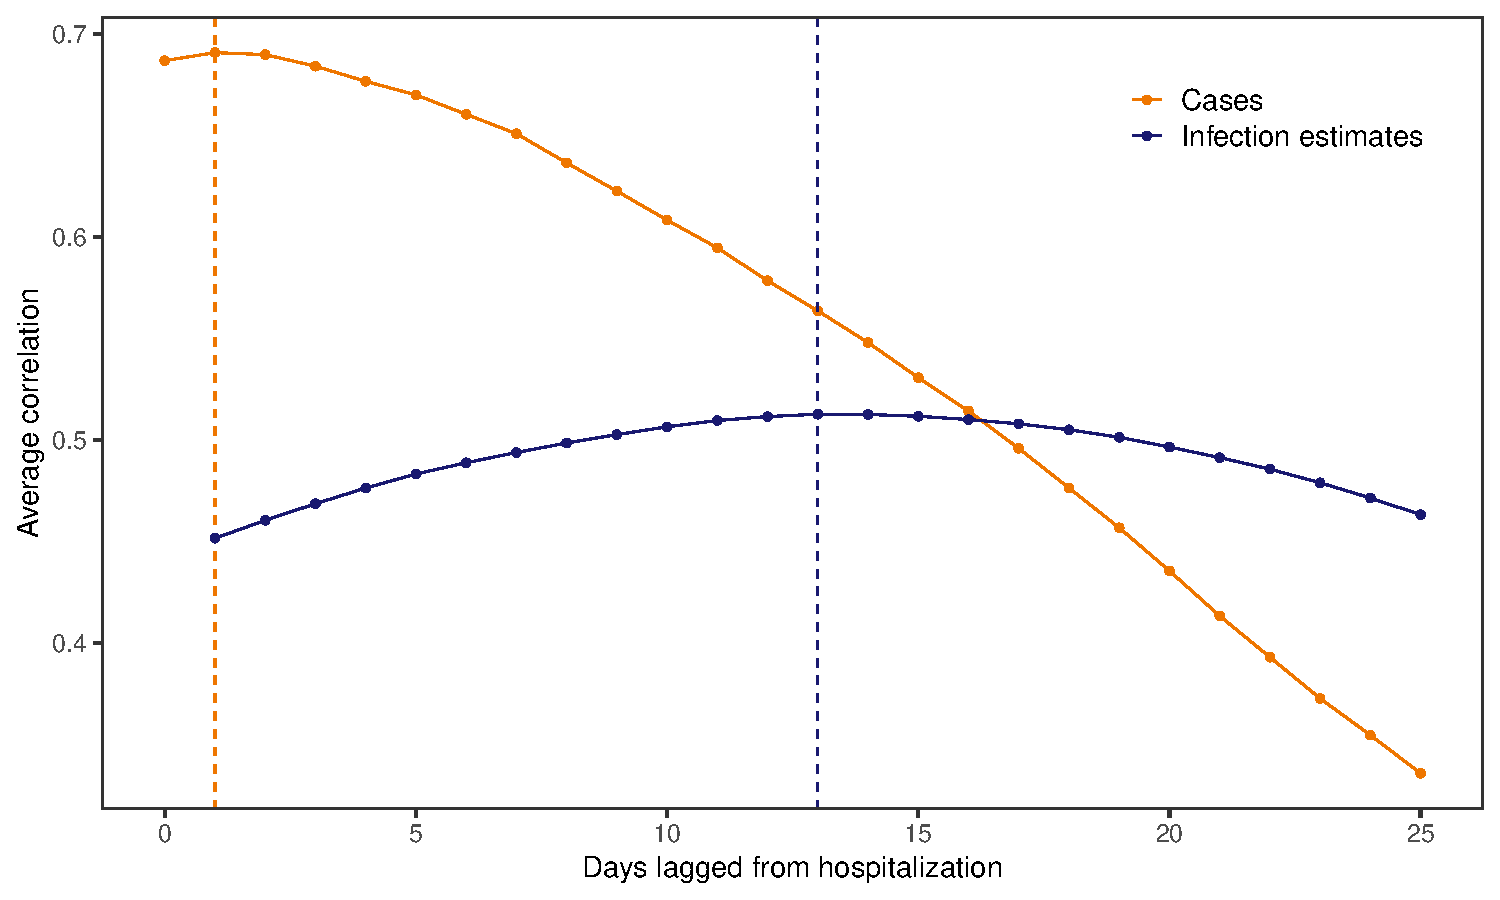
\includegraphics[width=.8\textwidth]{infect_case_hosp_lag_corr_F24.pdf} 
    \caption{Lagged Spearman's correlation between infection and hospitalization
    rates per 100,000 as well as between case and hospitalization rates per
    100,000. The averages shown are for each lag, across \US\ states and days
    over June 1, 2020 to November 29, 2021, and taken over a rolling window of
    61 days. Note that the infections, cases, and hospitalization counts are
    subject to a center-aligned 7-day averaging to remove spurious day of the
    week effects. The dashed lines indicate the lags for which the highest
    average correlation is attained.}
    \label{fig:infect_case_hosp_lag_corr}
\end{figure}

\begin{figure}[!tb]
\centering
    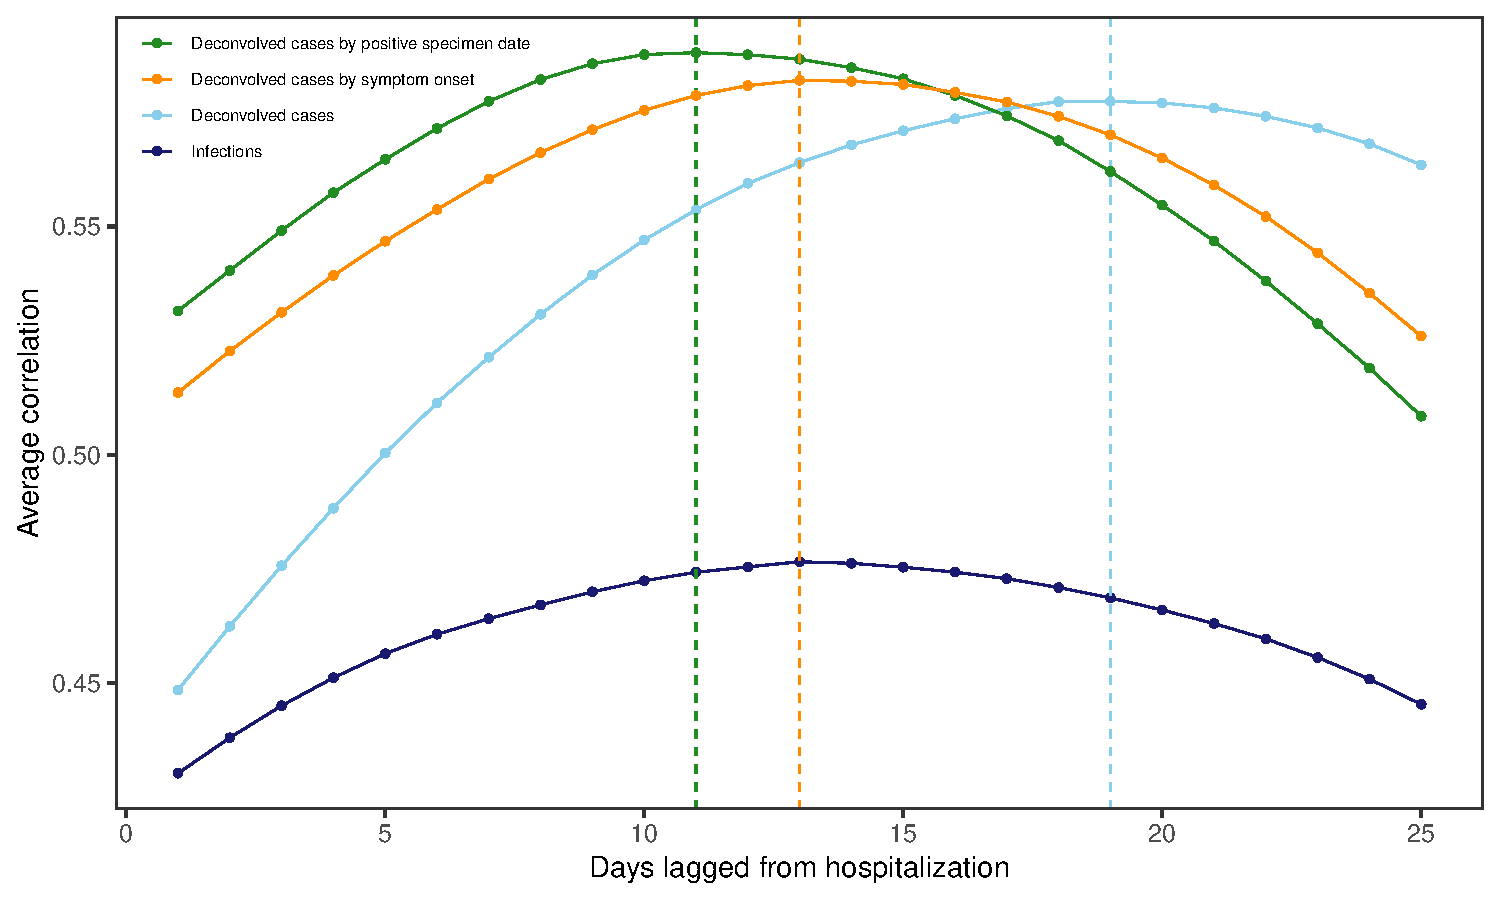
\includegraphics[width=.8\textwidth]{adj_unadj_pi_no_inc_hosp_lag_corr_F24.pdf} 
    \caption{Lagged Spearman's correlation between the infection and
    hospitalization rates per 100,000 averaged for each lag across \US\ states
    and days over June 1, 2020 to November 29, 2021, and taken over a rolling
    window of 61 days. The infection rates are based on the counts for the
    deconvolved case and infection estimates as well as the reported infections
    by symptom onset and when the report is symptom onset. Note that each such
    set of infection counts is subject to a center-aligned 7-day averaging to
    remove spurious day of the week effects. The dashed lines indicate the lags
    for which the highest average correlation is attained.}
    \label{fig:adj_unadj_sym_hosp_lag_corr}
\end{figure}

\begin{landscape}
\thispagestyle{empty}
\begin{figure}[!tb]
    \centering
   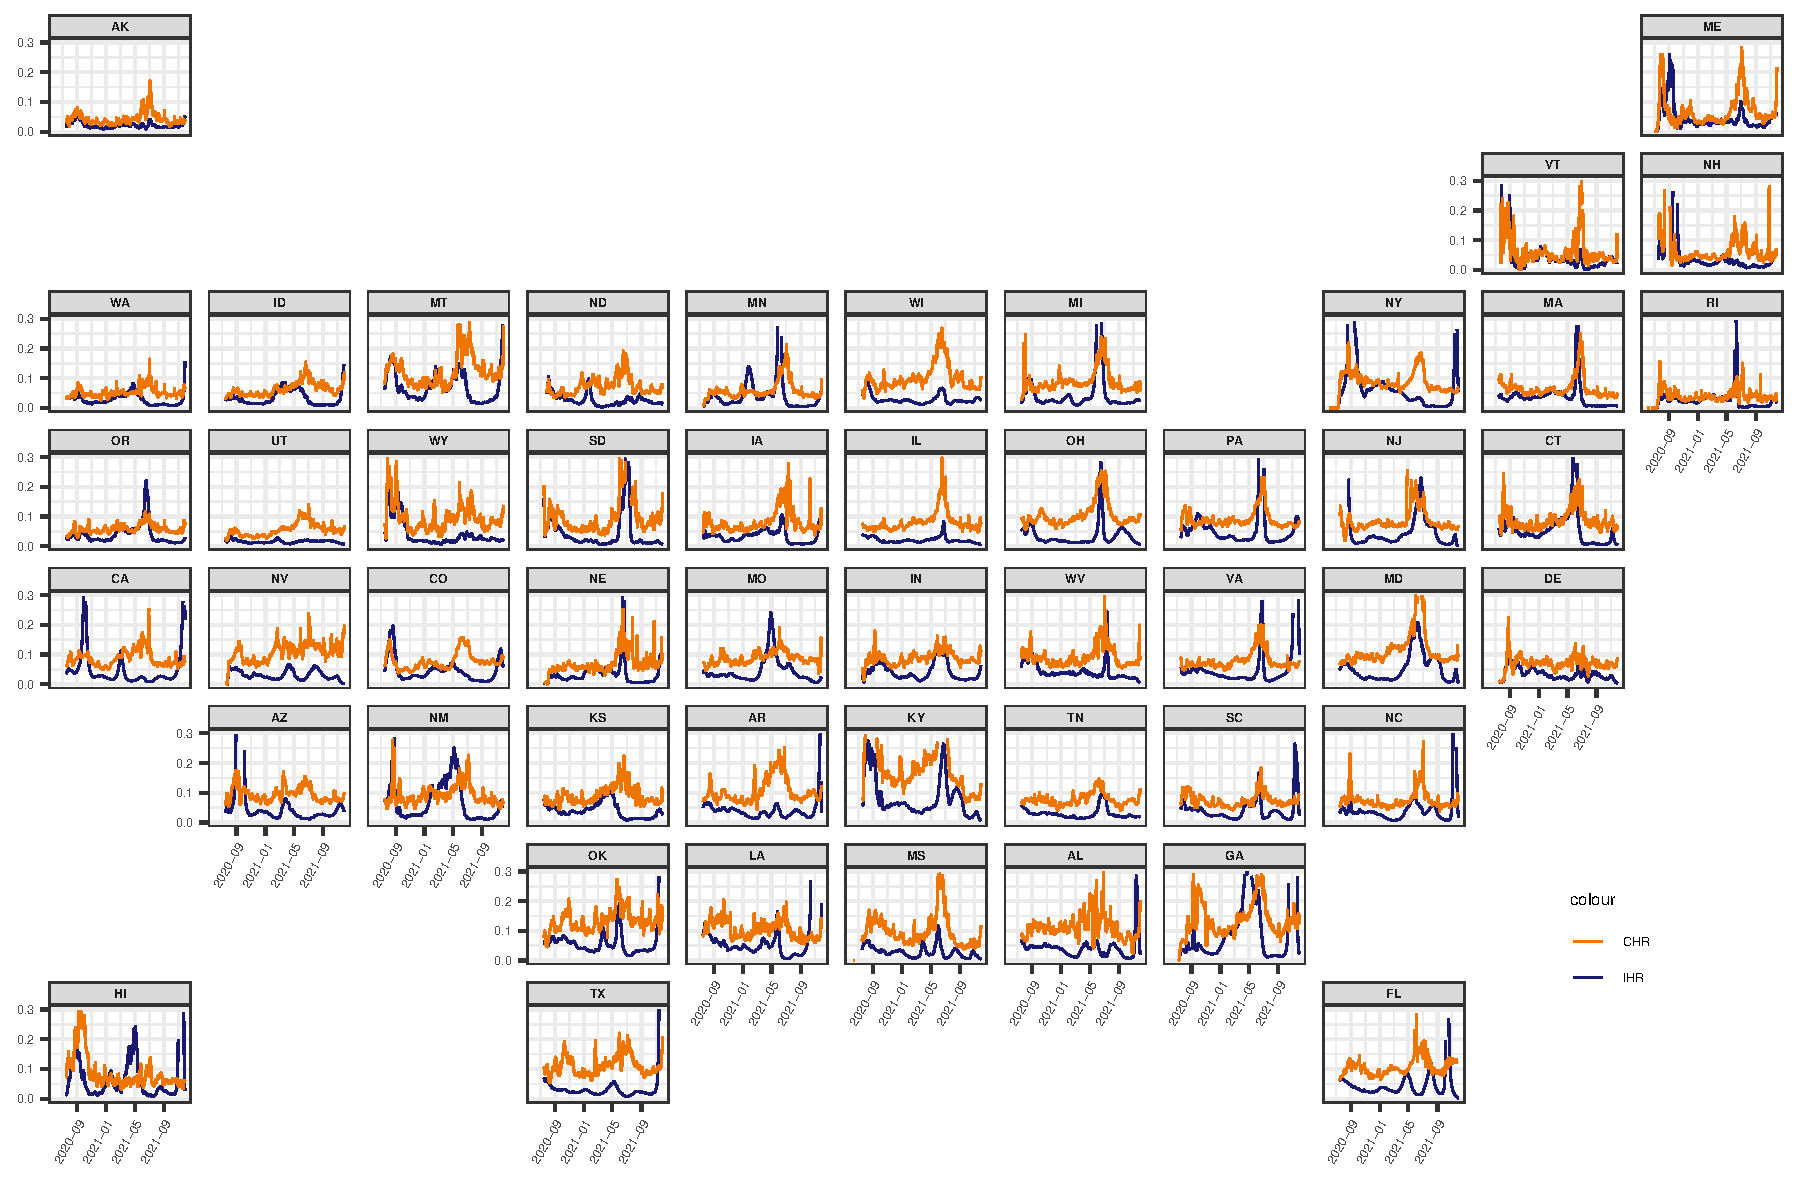
\includegraphics[width=.99\linewidth]{IHR_7dav_F24.pdf}
    \caption{Time-varying IHR and CHR estimates for each state from June 1, 2020
    to November 29, 2021, obtained using the corresponding optimal lag from the
    systematic lag analysis. Note that the infection, case, and hospitalization
    counts are subject to a center-aligned 7-day average to remove spurious day
    of the week effects. Also note that the different starting points across
    states are due to the availability of the hospitalization data.}
    \label{fig:IHR_7dav}
\fillandplacepagenumber
\end{figure}
\end{landscape}

\subsection{Disease burden and viral transmission}

From reconstructing the time series of COVID-19 infections per $100,000$
population for each \US\ state from June 1, 2020 to November 29, 2021, we observe
rates of infections that vary in intensity and disease burden across space and
time (\autoref{fig:state_infect_est},
 \autoref{fig:six_state_est}).  
 Most states present at least two major spikes in infections - the first starts in the fall of 2020 
 and extends into the winter season, while 
 the second starts in the late summer of 2021 and proceeds into the mid-fall. These represent major 
 waves driven by the Ancestral and Delta variants.
Similar patterns in the major surges of infections are observed in nearly all states, though to varying
 degrees. In general, greater similarities
in the strength and magnitude of outbreaks are found to emerge in the clusters of
states that border each other.

To avoid encroaching upon possible boundary issues with ending the estimation during a time of volatility
 (the period of the Delta-Omicron transition), 
we focus on the infection estimates prior to November 1, 2021.
The largest observed outbreaks prior to this time were observed in the late summer or early fall of 2021
in Georgia, Louisiana, Idaho, Montana, and Wyoming which suggests a similar spread of the virus in
small clusters of states that are in close geographic proximity. During this time, the two states that
have the attain the highest rate of infections per 100,000 on single day are Georgia with
about $451$ infections per 100,000 on August 15, 2021 (95\% confidence interval:
$[334, 567]$) and Idaho with $451$ on September 7, 2021 (95\%
confidence interval: $[312, 590]$). These are closely followed by Montana with $432$ on 
September 8, 2021 (95\% confidence interval: $[282, 581]$), Louisiana with $431$ on July 20, 2021
(95\% confidence interval: $[252, 610]$), and Wyoming with $350$ on November 13, 2020
(95\% confidence interval: $[256, 444]$).

Prior to the Delta wave, the state that has the
highest rate of infections per 100,000 on single day is Louisiana with about
358 infections per 100,000 on July 3, 2021 (95\% confidence interval:
$[177, 539]$), followed by Wyoming with 349 on November 13, 2020 (95\%
confidence interval: $[407, 546]$), South Dakota with 342 infections per 100,000 on July 3, 2021 
(95\% confidence interval:$[177, 539]$), and Illinois with 340 infections per
 100,000 on July 3, 2021 (95\% confidence interval:
$[177, 539]$). During this time, 74\% of the top rates for each state were observed in the
 late fall or winter of 2020.

The period of lowest viral transmission is observed in the summer and fall of 2020. 
During this time, the state of New Hampshire achieves the lowest weekly rate of infections 
of 0.01 infections per 100,000 for the week of September 13, 2020. In the summer of 
2020, Vermont maintains a rate under 10 infections per 100,000 from the week of June 1, 2020 to 
August 30, 2020, which is the longest continuous stretch observed for any state.

From a brief inspection of the geo-contiguous states, we can observe similar patterns in
surges and periods of waning over time, suggesting that states who share similarities in
climate and topography performed similarly to each other. More precisely, we can observe
neighboring states such as New Hampshire and Massachusetts or Idaho and Montana that
present waves that mirror each other in amplitude and timing. 

Interestingly, the two states that are geographically removed from the
contiguous United States, Alaska and Hawaii, tend to perform quite differently
from each other later in the pandemic. Alaska generally presents significantly greater rates of
infections than Hawaii especially during the Delta era. This suggests that
it is not so much the non-contiguity aspect as it is other distinguishing
factors that lead to lower infection rates.


%\subsection{Sensitivity analysis}
% This section is under construction
%The infection estimates exhibit modest changes under different assumptions about the
%variant-specific incubation periods, the construction of the delay distribution (the
%window size for the considered onset dates), the fraction of new infections over time, and
%the population estimates (see Supplementary Materials Section X). 
% Potentially compare ww a_t ratios over the time period as well (ie. do they fall in the confidence bands for a_t estimates
% from the ss model)?
% \attn {Add a sentence or two about what is meant by modest changes... Did any of these result in noticeably higher or lower (biased) estimates of infections? To what extent (ie. an additional X infections)? For what states?}
% Do these sensitivity analyses + update this link accordingly.

\section{Discussion}

We obtained retrospective estimates of daily incident infections for each \US\
state for June 1, 2020 to November 29, 2021. 
Our infection estimates suggest that the pandemic has an impact
in states earlier and at a larger scale than is indicated by cases. Since
case reporting is not consistent across time and states, case counts
underestimate the true number of infections and, hence, the impact of the
pandemic \citep{cdc2022estimated, simon2022inconsistent}. For example, some
states report the number of individuals tested rather than the numbers of tests
performed \citep{schechtman2020counting, chitwood2022reconstructing}.
Additionally, while the definition of a confirmed COVID-19 case tends to be fairly
uniform across the United States due to general adherence to the 
CSTE case definitions, state reporting standards have been known to vary 
\citep{cste2020, delphiepidata2020}. 
For instance, there may be inconsistencies across locations if some cases
are labelled as confirmed based on positive antigen tests instead of PCR
tests \citep{covidtracking2021}. 
% As well, the definition of a case and related terminology can change
% or evolve over time as more information becomes available.  

We observe outbreaks in infections that are difficult to detect from cases
alone such as the Delta wave in New Jersey, Connecticut, and Maryland. 
This suggests that cases paint an incomplete 
picture of the pandemic, especially when outbreaks are largely driven by 
unreported infections. Furthermore, since case report dates generally follow symptom and infection
onset, cases are a fundamentally flawed indicator of disease burden because they
have a built-in temporal bias. This is in addition to other biases from
differences in reporting across states (such as temporary bottlenecks due
influxes of data or more persistent processing issues that increase the average
time from case detection to report \citep{wash2020dash, dunkel2020covid19}. 
Furthermore, no indication of uncertainty is provided for even the gold standard case estimates
\citep{delphiepidata2020}. 
Thus, while reported cases provide an indication of the trajectory of the pandemic, it
is a delayed and incomplete version. Estimating the new number of infections by
symptom or infection onset date would more closely align with the definition of
incidence as we know it \citep{jahja2022real}.

From the correlation analysis between daily infection estimates and
hospitalizations, a lag of 13 days gives the maximum average correlation 
across states. This is in agreement with the early estimates of the average time from
infection to hospitalization of 9.7 days (95\% CI: $[5.4, 17.0]$) for
cases reported in January, 2020 in Wuhan, China as well as with estimates from
across the pandemic in the UK that ranged from an average of 8.0 to 9.7
days (more precisely, 8.0 days (95\% interval: $[2.7, 18.5]$) for the first
wave to 9.7 days (95\% interval: $[4.1, 19.6]$) for the second wave,
\citep{ward2021understanding}). However, we should note the first study is based
on a small sample size for outbreak cases reported well before our study start
date. As well, both sets of estimates depend upon the healthcare system and the
population structure, amongst other things \citep{ward2021understanding}.
Nevertheless, their relative agreement with our estimate of 13 days for the \US\
states lends some credence to of our results. 

While we computed and compared CHRs and IHRs for all states, 
it is important to note that both
likely to vary within states and depend on confounding variables such as
 age and the presence of major comorbidities \citep{russell2023comorbidities}.
 Therefore, it would be beneficial to account for such variables in their
 calculations by, for example, stratifying infections and hospitalizations by
 age to produce age-specific estimates of the IHRs for each state (similar to
 \citealp{fox2023disproportionate} though with the additional element of being
 time-varying). We strongly believe this would be a worthwhile direction to
 pursue in future work should the necessary information be available. 

The remainder of our discussion consists of an in-depth look into the advantages and
limitations of our approach and of other comparable approaches, followed by a
high level summary of our work and its major contributions. 

Our approach offers a number of advantages.
% The development 
% of a way of modelling immunity and space-time-specific reporting ratios based on 
% seroprevalence data.
% Similar phrase on line 1268, though we may want to emphasize that point up here.
% To the best of our knowledge, no other modelling approach has been used to 
% reconstruct the infection time series
%for every state over as much of the COVID-19 pandemic as in this study. %%
%Furthermore, 
For instance, we aim to incorporate as much state-specific information as
possible when deriving our estimates. By using state case, line list, and
variant circulation data, we are able to construct incubation and delay distributions
that are unique for each state. By using time-varying and state-specific
seroprevalence data, we are able to allow the reporting ratio to vary over both
time and state, which is an advantage over such ratios that are non-time varying
but state-specific and those that are time-varying but the same for all states
\citep{unwin2020state, uga2020covid19}. 
Existing approaches that use the delay distribution to generate infection
estimates often only construct one delay distribution that is used for all
states \citep{chitwood2022reconstructing, jahja2022real}. That is, they operate
under the assumption of geographic invariance, where it is assumed that all
states have the same patterns of delay from onset to case report,
which is unlikely to be true due to differences in reporting pipelines, pandemic
response, and variants in circulation, amongst other things. 

Another major limitation of these existing approaches to derive infections 
is that they do not to account for reinfections. 
Now, it may be contended that reinfections do not account for a
substantial fraction of the infections until later in the pandemic, so they are
not absolutely necessary to include in the earlier stages of the pandemic.
Still, at no stage did infection confer lifelong immunity.
Rather antibody levels and immunity are known to wane over time. 
And we believe it is important to account for such defining characteristics of the virus when
tracking infections over time. Therefore, we account for reinfections and the waning
of detectable antibody levels in our custom antibody prevalence model. However, we 
acknowledge that the extent to which each of these are accounted for could be
improved upon in future work. 

Since the waning of immunity is likely to be variant-dependent
\citep{pooley2023durability}, it follows that our model waning parameter may be better
posed as a mixture of parameters for different variants with weights determined
by the proportion of the variants circulating at the time in the state. Related
to this is the issue of how newer variants may escape detection
\citep{nih2022assessing, fda2023sars}. While in a retrospective analysis where
finalized data is used this is less likely to be an issue, this could very well
pose a problem for real-time estimates of infections.

Regarding reinfections, a major reason why we chose an end date of 
November 29, 2021 and ultimately decided to not tread into Omicron territory is because
 the Omicron variants come with substantial increase in the risk of reinfection in comparison
  to previous variants as Omicron has been shown to have an increased tendency towards
   immune escape \citep{wei2024risk, pulliam2022increased, eythorsson2022rate}. 
   So having quality reinfection data that is representative of each location under study is of the
    utmost importance for the Omicron era. 

While it would be ideal to use confirmed rates over time for each \US\ state, most states
 do not publicly report reinfection 
data over the entire time period we considered. So we have turned to 
suspected reinfection data over time for Clark County, USA, as that surveillance
is among the most detailed and reputable that we have found for the United States.
Nevertheless, using such localized data raises questions of representativeness
and the applicability of such estimates to Nevada and all other states.
Furthermore, this data has no information available beyond suspected third
infections, which imposes an irremediable bias. However, based on the third
infection data available there, we expect that the probability of being
reinfected more than three times is likely very low for time frame considered
and so the omission of these would impact our infection estimates to a minimal
extent. 

The vast majority of issues we encountered when trying to reconstruct the
infection time series for each state are due to an absence or a lack of data.
Such is the primary issue we had with the restricted line list. In comparison to
the number of JHU cases (which we are treating as a gold standard) for the same
release date, we noted there are about $10$ million cases that are unaccounted
for in the CDC line list. Moreover, the missingness does not appear to be random
and uniformly distributed across states. Rather it is unequally distributed,
suggesting that the dataset is likely biased. However, more information on the
cases that are missing versus present would be required to determine the extent
the missing cases led to a nonrepresentative, and therefore, biased sample, and
could be a topic of further study.

Seroprevalence data also runs the risk of being nonrepresentative of the
intended population \citep{bajema2021estimated}. For example, in the blood donor
dataset some states have region specific-estimates, which clearly do not stand
for the entire state. Another source of systematic variation is in the
characteristics of the individuals who opt for blood tests versus those who do
not. For instance, there may be a healthy user bias, in which a number of those
who opt for blood tests are generally more inclined to partake in proactive
healthy behaviors (such as checking on basic health markers by taking an annual
blood test) than those who do not \citep{parsley2018blood}. Alternatively, a
number of individuals may be recommended for blood tests by their doctors due to
signs of ill-health (ex. mineral deficiencies or underlying medical
conditions). The extent that each such bias persists depends on the purpose of
the blood test and whether it was used as a proactive or reactive medical tool.
Since such information is unavailable to us, all we can conclude is that
participant-driven sources of bias impact the seroprevalence samples to an
undetermined extent. There are additional concerns about the performance of
antibody testing for individuals with mild or asymptomatic disease as well as about
the loss of immunity over time \citep{kaku2021performance, seow2020longitudinal,
ibarrondo2020rapid}.

In this work, we do not attempt to directly address infection underascertainment
due to the increase in asymptomatic infections across variants
\citep{pho2023covid19}. We simply note that this would likely pose a greater
problem later in the pandemic, particularly after the Delta era
\citep{fan2022sars}. We hope that such infections would be largely represented
by the seroprevalence and reinfection estimates, but there is undoubtedly
increasing reliance on such estimates to be able to do this over time (owing to
the simultaneous decline in the reporting cadence and the apparent rise in
asymptomatic infections over time) \citep{oph2022covid, garrett2022high,
blauer2022reduce, ren2021asymptomatic}. Consequently, there is an increasing
uncertainty over time that is not captured by the model or the estimates.   

Due to such concerns with the seroprevalence data, one further area of research
is on investigating the utility of various sources to estimate the incidence of
infections. Intuitively, one might expect that leveraging data from multiple
sources would likely lead to more accurate and stable estimates than those from
using one source. Wastewater surveillance data is one
promising source that may be complementary to seroprevalence data, especially
when testing is low \citep{mcmanus2023predicting}. However, there has been
limited success in predicting incidence using such data. The extent that
wastewater concentration data is a useful in estimating COVID-19 incidence is
unclear owing to problems with viral occurrence and detectability in wastewater
that render detection inconsistent across locations (ex. due to temperature,
per-capita water use, and in-sewer travel time) \citep{mcmanus2023predicting,
hart2020computational, li2023correlation}. Sentinel surveillance streams for
influenza-like illness or acute respiratory infection may provide decent proxies
for COVID-19 incidence, especially when testing for mild cases of COVID-19 is
diminishing or has ceased completely. Finally, alternative surveillance streams
(potentially outside of public health) such as those from surveys, helplines, or
medical records could potentially be integrated if they provide at least a rough
indication of the disease intensity over time \citep{ecdc2020strategies}.

Overall, we adopt a relatively simple deconvolution-based approach and devote
much of our efforts to tailoring our approach to the available data. A
major result of this is the development of a way of to model the waning
of detectable antibody levels and space-time-specific reporting ratios based on
 seroprevalence data. In a way, our approach is built for the data rather than trying to force 
 the data to fit to an existing approach. However, our model is only as good as the quality and
the quantity of the data provided to it. In our case, the lack of data is both a barrier to entry
and a continual roadblock. The assumptions we are required to make as a
consequence of this clearly limit the generalizability and call into question
the reliability of the results. So while we highlight some interesting trends and
numerical findings, these results are not definitive, but rather exploratory and
intended to stimulate discussion on the challenging task of estimating
infections. Despite these limitations, we are encouraged by the ability to use
routine data to produce sensible estimates of infections in the United States and the
plausibility of the apparent geospatial and temporal trends. 
 
Our approach is predicated upon having case, line list, viral circulation, and
seroprevalence data for each state, all of which are readily available (or
available upon request in the case of restricted line list data). As a result of
this, we are able to demonstrate the feasibility of estimating COVID-19
infections at the state level by using standard sources of data. 

Our framework is quite versatile as it lends itself to more localized, county or
community level estimates, or globalized, country-specific estimates.
Fundamentally, to produce estimates of infections for different geographic
regions, one would simply need to input the required data and re-run the code
pipeline. In this way, one could readily adapt our approach to generate
estimates for the provinces in Canada or the regions in England.

Well-informed, localized estimates of COVID-19 infections over time can help us
to have a more clear and comprehensive understanding of the course of the
pandemic. Such estimates contribute important information on the timing and
magnitude of disease burden for each location and they highlight trends that may
not be visible from case data alone. Therefore, our infection estimates provide
key information for the ongoing debate on the true size and impact of the
pandemic.



\subsection*{Acknowledgements}

% Required Gisaid acknowledgement
We gratefully acknowledge all data contributors, i.e., the Authors and their
Originating laboratories responsible for obtaining the specimens, and their
Submitting laboratories for generating the genetic sequence and metadata and
sharing via the GISAID Initiative \citep{elbe2017data}, on which this research
is based.

%\bibliographystyle{naturemag} %% Change back to numeric references in line with requirements for Nature Communications articles (see pg 3 fro here: https://www.nature.com/documents/ncomms-formatting-instructions.pdf)
\bibliographystyle{rss}

\newpage
\bibliography{bibliography.bib}

\newpage
% Eventually make the supplement a separate document with its own title page 
\beginsupplement
\title{\supptitlefont Online Supplement}
\maketitle

\section{Additional information about dataset used or estimation methodology}

\subsection{Table on the percent pairwise occurrence of events in the CDC line list}
\begin{table}[h!]
\begin{tabular}{|l|l|l|}
\hline
\textbf{Order of events}                              & \textbf{Percent pairwise occurrence}                                                                                    & \textbf{Handling}                                                                                                                                                                                                                                                                                                                                                          \\ \hline
IO $\rightarrow$ SO $\rightarrow$ PS $\rightarrow$ RE & \begin{tabular}[c]{@{}l@{}}PS $\geq$ SO: 97.1 \\ PS = SO: 33.6\\ PS \textgreater RE: 1.74\\  PS = RE: 14.6\end{tabular} & \begin{tabular}[c]{@{}l@{}}This is the idealized order of events and so we \\ built the current support sets for \\ SO $\rightarrow$ PS and PS $\rightarrow$ RE \\ delay distribution constructions around this \\ such that IO comes first by construction, \\ SO typically precedes PS, but may be the same \\ or come before, and RE comes after PS and SO\end{tabular} \\ \hline
IO $\rightarrow$ PS $\rightarrow$ SO $\rightarrow$ RE & \begin{tabular}[c]{@{}l@{}}PS \textless SO: 2.91 \\ SO $\leq$ RE: 99.3 \\ SO \textless RE: 86.1\end{tabular}            & \begin{tabular}[c]{@{}l@{}}Allowed for negative delays up to the largest \\ non-outlier value for the 0.05 quantile of delay\\ from PS to SO by state\end{tabular}                                                                                                                                                                                                         \\ \hline
IO $\rightarrow$ PS $\rightarrow$ RE $\rightarrow$ SO & \begin{tabular}[c]{@{}l@{}}RE \textless SO: 0.7 \\ RE \textless PS: 1.7\end{tabular}                                    & \begin{tabular}[c]{@{}l@{}}Nothing because current handling of the CDC \\ of the line list ensures that the most concerning \\ cases are handled where \\ SO = PO = RE, SO = RE and PO = RE\end{tabular}                                                                                                                                                                   \\ \hline
\end{tabular}
\caption{Percent pairwise occurrence for the different permutations of events considered in the restricted CDC line list. The abbreviation IO stands for infection onset, SO is symptom onset, PS is positive specimen, and RE is report date. We consider a restricted set of permutations because we assume that IO must come first and that PS must precede report date for a case to be legitimate. Finally, the underlying assumption for the percent pairwise occurrence calculations is that the cases must have both elements present (not missing).}
\label{order_events_table}
\end{table}

\subsection{State space representation of the antibody prevalence model}\label{supp:ssapm} 

The antibody prevalence model from \autoref{eq:waningpr} is conceptualized
as a Gaussian state space model (as in \citealp{durbin2012time, helske2017kfas}).

In general, for $t = 1, \dots, n$, let $\alpha_t$ be the $m \times 1$ vector of latent
state processes at time $t$ and $y_t$ be the $p \times 1$ vector of observations
at time $t$. Under the assumption that $\eta$ is a $k \times 1$ vector, the
form of the linear Gaussian state space model is 
\begin{align}
y_t &= Z\alpha_t + \epsilon_t, \qquad \epsilon_t \sim N(0, H_t) \label{eq:ss1}\\
\alpha_{t+1} &= T_t\alpha_t + R_t\eta_t, \quad \eta_t \sim N(0, Q_t) \label{eq:ss2}
\end{align}
where $\alpha_1 \sim N(a_1, P_1)$ and 
there is independence amongst $\alpha_1$, $\epsilon_t$ and $\eta_t$
\citep{helske2017kfas, durbin2012time}. For notational
compactness, we let $\alpha = \left ( \alpha_1^\top, \dots, \alpha_n^\top \right )$
and $y = \left ( y_1^\top, \dots, y_n^\top \right )$.

The observation equation can be viewed as a linear regression model with the
time-varying coefficient $\alpha_t$, while the second equation is a first-order
autoregressive model, which is Markovian in nature \citep{durbin2012time}. 

The underlying idea behind the two equations is that we are assuming that the
system evolves according to $\alpha_t$ (as in the second equation), 
but since those states are
not directly observed, we turn to the observations $y_t$ and use their
relationship with $\alpha_t$ (as in the first equation) to drive the system
forward \citep{durbin2012time}. So the objective of state space modeling is to
obtain the latent states $\alpha$ based on the observations $y$ and this is
achieved through Kalman filtering and smoothing. 

Kalman filtering gives the following one-step-ahead predictions of the states
\begin{align*}
a_{t+1} &= \E[\alpha_{t+1}\given y_t, \dots, y_1] 
\end{align*} with covariance,
\begin{align*}
P_{t+1} &= \Var(\alpha_{t+1} \given y_t, \dots, y_1).
\end{align*}
Then, the Kalman smoother works backwards to the first time to give
\begin{align}
\hat{a}_t &= \E[\alpha_{t}\given y_n, \dots, y_1] \label{eq:hatat}\\
V_t &= \Var(\alpha_{t}\given y_n, \dots, y_1). \label{eq:Vt}
\end{align}
The filtering and smoothing steps are based on recursions that are described in
Appendix A of \citet{helske2017kfas} as we use the R package KFAS to estimate
our model.

% For our situation, the Kalman filter and smoothing approach offers a number of
% advantages over the penalized regression approach. Perhaps most notably,
% the parameters are estimated all at once (so cross validating for model
% parameter tuning is not necessary). Another major benefit is that it can handle 
% unevenly spaced time series (refer to \citealp{durbin2012time} for further details).

To express the antibody prevalence model in state space form, we define
 the components in Equations \ref{eq:ss1} and \ref{eq:ss2} as follows:

% Probably move the below specification to the appendix

\begin{alignat*}{3}
R &= \begin{bmatrix}
1 & 0  \\ 
0 & 1 \\ 
0 & 0 \\ 
0 & 0 
\end{bmatrix} &\qquad 
Z &= \begin{bmatrix}
1 & 0 & 0 & 0 \\ 
0 & 1 & 0 & 0 
\end{bmatrix} &\qquad 
H_m &= \begin{bmatrix} %%
w_{m,c}\sigma^2_o & 0 \\ 
0 & w_{m,b}\sigma^2_o
\end{bmatrix} \\
\alpha_m &= \begin{bmatrix}
s_{m}\\
a_m\\ 
a_{m-1}\\ 
a_{m-2}
\end{bmatrix} & 
T_m &= \begin{bmatrix}
 \gamma & C_{m-1}^m z_m & 0 & 0\\ 
 0 & 3 & -3 & 1 \\ 
 0 & 1 & 0 & 0\\ 
 0 & 0 & 1 & 0
\end{bmatrix}  & 
Q &= \begin{bmatrix} 
\sigma^2_s & 0  \\ 
0 & \sigma^2_a
\end{bmatrix} \\
a_1 &= \begin{bmatrix}
\tilde{s}_{1}\\ 
\tilde{a}_1\\ 
\tilde{a}_1 \\
\tilde{a}_1
\end{bmatrix} & 
P_{1} &= \begin{bmatrix}
\sigma^2_{\tilde{s}_{1}} & 0 & 0 & 0 \\ 
0 & \sigma^2_{\tilde{a}_1} & 0 & 0\\ 
0 & 0 & \sigma^2_{\tilde{a}_1} & 0 \\ 
0 & 0 & 0 & \sigma^2_{\tilde{a}_1}
\end{bmatrix} 
\end{alignat*}
where $\sigma^2_o$ is the variance of observations,
$\sigma^2_s$ is the variance of the seroprevalence estimates, 
and $\sigma^2_a$ is the trend variance. Since we expect the 
inverse ratios to be more variable than the seroprevalence estimates, 
we enforce that the estimate of $\sigma^2_a$ is a multiple of 
$\sigma^2_s$. Letting the subscripts $b$ and $c$ denote
the blood donor and commercial datasets, $w_{m,c}$ and $w_{m,b}$ are the
time-varying inverse variance weights computed from the commercial and blood
donor datasets, respectively. 

For each source, we compute the weights for the observed seroprevalence
estimates using the standard formula for the standard error of a proportion.
These weights are then re-scaled so they sum to the number of observed
seroprevalence measurements for the source. All days that are unobserved (i.e.,
lack seroprevalence measurements) are given weights of one. Finally, the ratio
of the average observed weights for the sources is used as a multiplier to scale
all of the weights for one source. For example, if the average weight of the
commercial source is double the average weight of the blood donor source (for an
arbitrary state), then we scale all of the weights in the commercial source
(including the ones) by two. The main purpose of this step is to ensure that
the source with a greater sample size contributes more weight in the model on
average. % Last sentence - Or is it simply that the source with larger
%weights on average will have more weight? 

The prior distribution for $\alpha_1$ is estimated using both data-driven constraints 
and externally sourced information. To obtain the initial value of the seroprevalence 
component, $\tilde{s}_{1}$, we extract the first observed seroprevalence measurement from 
each source, round down to two decimal places, and take the average to be $\tilde{s}_{1}$. 
The corresponding initial
variance estimate, $\sigma^2_{\tilde{s}_{1}}$, is taken to be the mean of the standard
errors of the two seroprevalence estimates. For all of the initial values of the trend 
components, we use the inverse of the ascertainment ratio estimate as of June 1, 2020 
for each state from Table 1 in \citet{unwin2020state} and denote this by $\tilde{a}_1$. The
initial variance estimate of $\sigma^2_{\tilde{a}_1}$ is based on the variance implied 
by the given inverse ascertainment ratio distribution.
% standard deviation implied by the interval in that table.  
% Update this last sentence if end up going with the standard deviation implied by the interval in Table 1
% instead of the variance implied by u_m ~ Beta(12,5) from the unwin2020state paper

The initial $\sigma^2_o$ is taken to be the average of the estimated variances
from the linear models for the sources where the observed seroprevalence
measurements are regressed on the enumerated dates. The initial value of 
the multiplier is set to be $100$ for all states. The $\sigma^2_s$ and $\gamma$ 
values are fixed and from averaging the estimated values for all states on the real line
(obtained under the starting conditions $\sigma^2_s = 0.000003$, $\gamma = 0.99$,
and $\sigma^2_o$ as described).

Following the maximum likelihood estimation of the two non-fixed parameters
we use the Kalman filtering and smoothing to obtain the
smoothed estimates of the weekly inverse reporting ratios and
their covariance matrices as shown in Equations \ref{eq:hatat} and \ref{eq:Vt}.
Forwards and backwards extrapolation is then used to estimate the ratios and covariance
outside of the observed seroprevalence range \citep{durbin2012time}, followed by linear 
interpolation to fill-in estimates for each day in our considered time period. 
After we obtain one vector of inverse reporting ratios for each state in this
way, we take each inverse reporting ratio and multiply it by the corresponding
deconvolved case estimate (that has undergone linear interpolation to correct
instances of $0$ reported infections) to obtain an estimate of new infections.
We are able to convert these numbers of infections to
infections per $100,000$ population by simple re-scaling (enabled by the fact
that normality is preserved under linear transformations).

The $50$, $80$, and $95\%$ confidence intervals are constructed by taking a
Bayesian view of the antibody prevalence model (refer to \ref{supp:bayeswaning} 
for the Bayesian specification of the model). 
That is, for each time, $t$, we obtain an estimate of the
posterior variance of $a_t$, apply the deconvolved case estimate as a constant
multiplier, and then use resulting variance to build a normal confidence
interval about the infection estimate. We additionally enforce that the lower
bound must be at least the deconvolved case estimate for the time under consideration.


\subsection{Bayesian specification of the antibody prevalence
model}\label{supp:bayeswaning} 
In brief, the antibody prevalence model where we let
$\beta = \left \{  \gamma, a_1,\dots, a_t \right \}$ and $X$ be the design
matrix, corresponds to a Bayesian model with prior 
\begin{align*}
    \beta \sim N \left( 0,  \frac{\sigma^2 }{ \lambda} \left( A^TD^TDA 
    \right)^{-1}  \right)
\end{align*} and likelihood 
\begin{align*}
    s|X,\beta \sim N \left( X\beta, \sigma^2W^{-1} \right),
\end{align*} where $A$ is indicator matrix save for the first column of $0$s 
(corresponding to $\gamma$), $D$ represents the discrete derivative matrix of 
order $3$, and $W$ is the inverse variance weights matrix. Then, the posterior 
on $a_t$ is normally distributed with mean 
\begin{align*}
    \left ( X^TWX + \lambda A^TD^TDA \right )^{-1}X^TWs
\end{align*} 
and variance 
\begin{align*}
    \sigma^2 (X^TWX + \lambda A^TD^TDA)^{-1}.
\end{align*}

\end{document}
